%======================================================================
\chapter{Literature Review}
%======================================================================
For a long time (until 2002), mean squared error (MSE) and peak signal to noise ratio (PSNR) were the common criteria for comparing the quality of a distorted image to a reference~\cite{Wang2004}. Although these metrics are intuitively explainable and computationally efficient, they are not well-correlated with human opinions~\cite{Wang2009,Wang2002}. Structural similarity was proposed to cover this gap~\cite{Wang2002a}. With the introduction of this criterion, many methods were proposed to measure the structural similarity, which a large number of them are based on image edges~\cite{Xue2014}.

For referenceless assessment, natural scene statistics (NSS) were the criterion of choice for many metrics. Ruderman~\cite{Ruderman1994} showed that natural images\footnote{``An image recorded from the physical environment with a camera that is sensitive to the visible spectrum of electromagnetic wave"~\cite{Liu2014a}} obey statistical regularities that are stable, regardless of the image content. So deviation from these regularities were exploited as a measure for distortion.

With the introduction of multiple distortion datasets, methods were proposed that tried to consider the simultaneous existence of multiple distortions in an image and extract features that describe their severity.

In this chapter we introduce the structural similarity criterion and two methods for its measurement. Then we review the approaches taken for NR IQA. The FR, RR, and NR algorithms proposed for IQA of multiply-distorted images are explained and analyzed in subsequent sections.
%-------------------------------------------------------------------
\section{FR Methods for Single Distortion IQA}
%------------------------------------------------------------------
Numerous researches in IQA were conducted for full reference assessment~\cite{lin2010perceptual}. Assuming a reference image, $r$, and its distorted version, $d$; computing the difference between $r$ and $d$ maybe the first approach that comes to our minds for comparing them. This is what MSE, PSNR, or RMSE do. For two grayscale images, $r$ and $d$:
\begin{equation}
    MSE(r, d) = \frac{1}{M\times N}\sum_{x=1}^M\sum_{y=1}^N(r(x, y)-d(x, y))^2
    \label{eq:mse}
\end{equation}
Where $M$ and $N$ are image dimensions. For two identical images, MSE will be zero and this is in accordance with our opinion: \emph{`` the quality perceived from two identical images is the same"}, but there are many cases that MSE is independent of image distortions; Fig.~\ref{fig:einstein} shows an example (figure from~\cite{Wang2004}).
\begin{figure}
     \centering
     \begin{subfigure}[b]{0.3\textwidth}
         \centering
         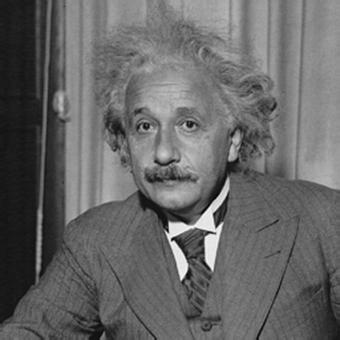
\includegraphics[width=\textwidth]{./figs/image003}
         \caption{Einstein's photo\\.\\.}
         \label{fig:einstein-orig}
     \end{subfigure}
     \hfill
     \begin{subfigure}[b]{0.3\textwidth}
         \centering
         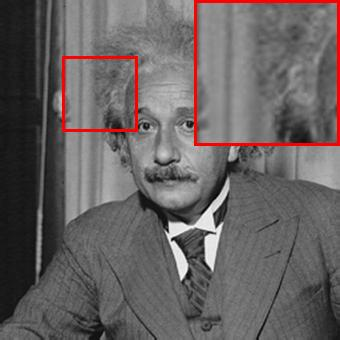
\includegraphics[width=\textwidth]{./figs/image003_bn}
         \caption{original image\\$MSE=0$\\$SSIM=1$}
         \label{fig:einstein-orig-s}
     \end{subfigure}
     \hfill
     \begin{subfigure}[b]{0.3\textwidth}
         \centering
         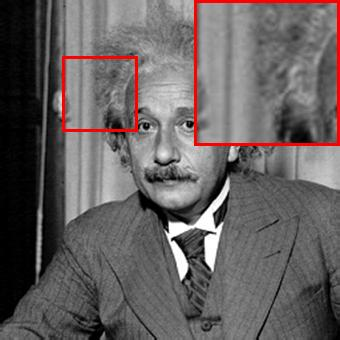
\includegraphics[width=\textwidth]{./figs/image0_bn}
         \caption{contrast change\\$MSE=144$\\$SSIM=0.913$}
         \label{fig:einstein-cc}
     \end{subfigure}
     \\
     \begin{subfigure}[b]{0.3\textwidth}
         \centering
         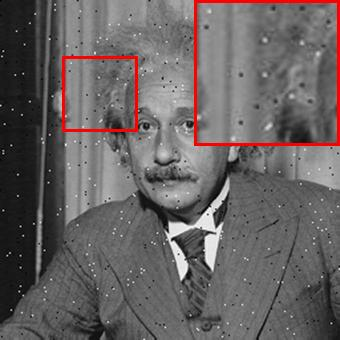
\includegraphics[width=\textwidth]{./figs/image009_bn}
         \caption{salt \& pepper noise\\$MSE=144$\\$SSIM=0.840$}
         \label{fig:einstein-sp}
     \end{subfigure}
     \hfill
     \begin{subfigure}[b]{0.3\textwidth}
         \centering
         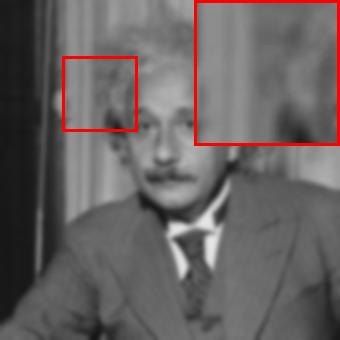
\includegraphics[width=\textwidth]{./figs/image011_bn}
         \caption{blur\\$MSE=144$\\$SSIM=0.694$}
         \label{fig:einstein-bl}
     \end{subfigure}
     \hfill
     \begin{subfigure}[b]{0.3\textwidth}
         \centering
         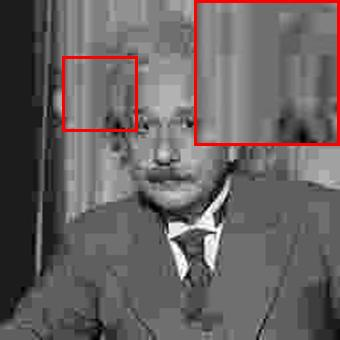
\includegraphics[width=\textwidth]{./figs/image013_bn}
         \caption{Jpeg quantization\\$MSE=144$\\$SSIM = 0.662$}
         \label{fig:einstein-jp}
     \end{subfigure}
        \caption{$MSE$ and $SSIM$ for different distorted versions of Einstein's photo.}
        \label{fig:einstein}
\end{figure}
We see different versions of the reference image in Fig.~\ref{fig:einstein-orig} with four artifacts ( the image in Fig.~\ref{fig:einstein-orig-s} is the reference, only magnified). MSE for the identical images equals zero (Fig.~\ref{fig:einstein-orig-s}), but in spite of the different visual quality of images in Fig.~\ref{fig:einstein-cc}-~\ref{fig:einstein-jp}, MSE is the same for all them, while a human observer prefers the image in Fig.~\ref{fig:einstein-cc} to the image in Fig.~\ref{fig:einstein-jp}.

MSE and similar approaches are based on ``error visibility". Wang and Bovik~\cite{Wang2002a} showed that the semantic information which we grasp from images are based on image structures. With a degradation in image structures we do not understand what we expect from a scene and perceive this as a low quality. They proposed a method, called `` SSIM~\cite{Wang2004}", for measuring the \underline{s}tructural \underline{sim}ilarity between two images. With the popularity of this method, researchers proposed other metrics for structural similarity and, as mentioned before, many of them are based on image edges. In what follows SSIM and one of the gradient based methods are explained.
%-------------------------------------------------------------------------------
\subsection{Structural Similarity}
%------------------------------------------------------------------------------
SSIM assumes that the structural similarity of two images is dependent on three factors: the correlation between the images, the luminance similarity, and the contrast similarity of the two image. That is, the more similar the two images are according to these criteria, the better is the quality of the distorted image. The abstract definition of SSIM for two grayscale images, $r$ and $d$, will be as follows:
\begin{eqnarray*}
\lefteqn{SSIM(r, d) = }\\
& & pixel\_wise\_correlation\times\\
& & luminance\_similarity\times\\
& & contrast\_similarity
\end{eqnarray*}
In SSIM, the contrast of an image is modeled with the variation in intensity values of pixels and luminance is modeled with the average of the values. If $I$ is an image with $N$ pixels, its luminance and contrast are represented as $\mu_I$ and $\sigma_I$, respectively, and obtained via the statistical definitions:
\begin{equation}
    \mu_I = \frac{1}{N}\sum_{x=1}^{N}I(x)
    \label{eq:mu}
\end{equation}
\begin{equation}
    \sigma_I = \sqrt{\frac{1}{N-1}\sum_{x=1}^N(I(x)-\mu_I)^2}
    \label{eq:sigma}
\end{equation}
Where, $I(x)$ is the value of the $x^{th}$ pixel of $I$. For obtaining the similarity of two numbers, authors used a similarity relation. The similarity of two numbers, $a$ and $b$, are represented as $sim(a, b, c)$, and defined as:
\begin{equation}
    sim(a, b, c) = \frac{2\times a\times b+c}{a^2+b^2+c}
    \label{eq:sim}
\end{equation}
Where $c$ is a constant for avoiding the instability of the fraction. Therefore, contrast and luminance similarity for $r$ and $d$ is obtained from~\ref{eq:c_sim} and~\ref{eq:l_sim}.
\begin{equation}
    contrast\_similarity(r,d)=sim(\sigma_r, \sigma_d, c)\in [0, 1]
    \label{eq:c_sim}
\end{equation}
\begin{equation}
    luminance\_similarity(r, d) = sim(\mu_r, \mu_d, c)\in [0, 1]
    \label{eq:l_sim}
\end{equation}
The correlation between two images are defined as the statistical correlation of the intensity values of the pictures. If $r(x)$ and $d(x)$ are the $x^{th}$ pixel from the $N$ pixels in $r$ and $d$, the correlation between $r$ and $d$ is obtained from the following equation:
\begin{equation}
    pixel\_wise\_correlation(r, d) = \frac{\frac{1}{N-1}\sum_{x=1}^N(r(x)-\mu_r)(d(x)-\mu_d)}{\sigma_r\times \sigma_d} \in [-1, 1]
    \label{eq:corr}
\end{equation}
For two identical images, SSIM will be equal to one. It is expected that it decreases with the deviation of the image. In Fig.~\ref{fig:einstein} we see that this occurs and SSIM distinguishes different perceived qualities. It must be mentioned that SSIM is computed for each corresponding $8\times 8$ window in the images and for pooling the scores of the windows into one score for the entire image, the SSIM values are averaged.
\subsection{Similarity of Gradient Magnitude}
Apart from SSIM, there are other metrics proposed for measuring the structural similarity. One of the approaches, is considering the edges of the image as a representative of image structures. Image gradients are known as good estimations of the edges~\cite{Gonzalez2008}. In location $(x, y)$ of image $I$, the gradient vector $\Vec{G}_I(x, y)$ has a horizontal and a vertical component, $g_h$ and $g_v$, respectively. The magnitude and direction of $\Vec{G}_I$ in $(x, y)$ are defined in relations~\ref{eq:gm} and~\ref{eq:gd} with respect to these components.
\begin{equation}
    GM_I(x, y) = \sqrt{g_v^2+g_h^2}
    \label{eq:gm}
\end{equation}
\begin{equation}
    GD_I(x, y) = tan^{-1}(\frac{g_v}{g_h})
    \label{eq:gd}
\end{equation}
The method GMSD~\cite{Xue2014} used $GM$ for measuring image distortions.
\begin{figure}
     \centering
     \begin{subfigure}[b]{0.3\textwidth}
         \centering
         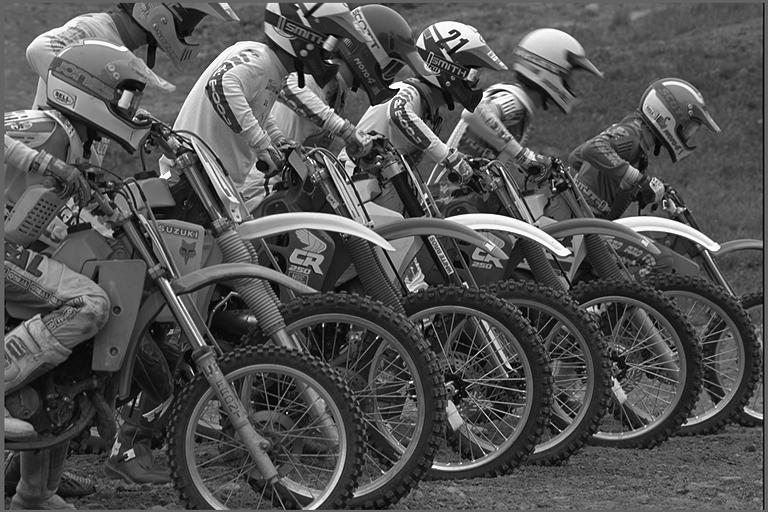
\includegraphics[width=\textwidth]{./figs/reference_gry}
         \caption{original image\\.}
         \label{fig:gmsd_ref_gry}
     \end{subfigure}
     \hfill
     \begin{subfigure}[b]{0.3\textwidth}
         \centering
         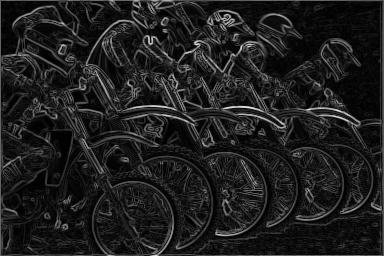
\includegraphics[width=\textwidth]{./figs/reference_mag}
         \caption{gradient magnitude of the original image}
         \label{fig:gmsd_ref_mag}
     \end{subfigure}
     \hfill
     \begin{subfigure}[b]{0.3\textwidth}
         \centering
         \fbox{
\includegraphics[width=0.9\textwidth]{./figs/reference_sim}}
         \caption{gradient magnitude similarity of the original image}
         \label{fig:gmsd_ref_sim}
     \end{subfigure}
     \\
     \begin{subfigure}[b]{0.3\textwidth}
         \centering
         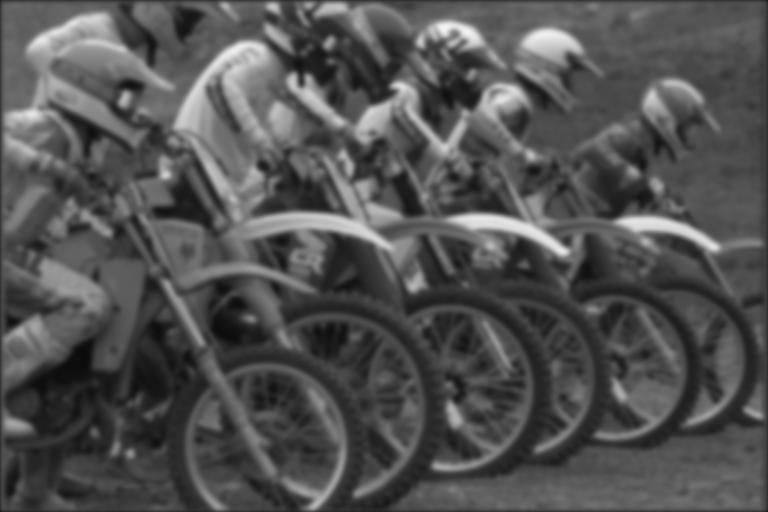
\includegraphics[width=\textwidth]{./figs/blur_gry}
         \caption{blurred image\\.}
         \label{fig:gmsd_blur_gry}
     \end{subfigure}
     \hfill
     \begin{subfigure}[b]{0.3\textwidth}
         \centering
         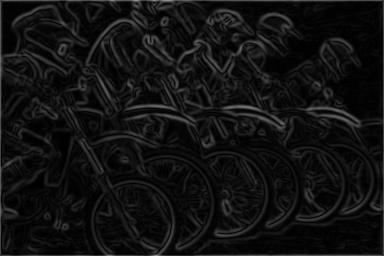
\includegraphics[width=\textwidth]{./figs/blur_mag}
         \caption{gradient magnitude of the blurred image}
         \label{fig:gmsd_blur_mag}
     \end{subfigure}
     \hfill
     \begin{subfigure}[b]{0.3\textwidth}
         \centering
         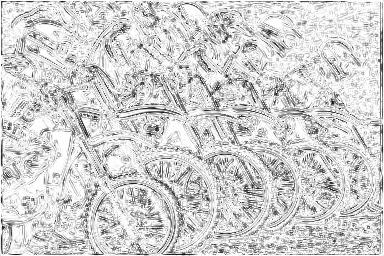
\includegraphics[width=\textwidth]{./figs/blur_sim}
         \caption{gradient magnitude similarity of the blurred image}
         \label{fig:gmsd_blur_sim}
     \end{subfigure}
     \\
     \begin{subfigure}[b]{0.3\textwidth}
         \centering
         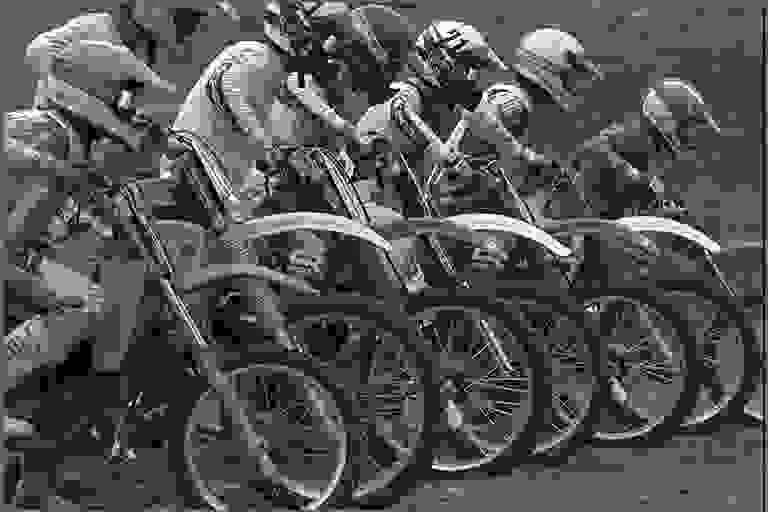
\includegraphics[width=\textwidth]{./figs/jpeg_gry}
         \caption{image with Jpeg artifact\\.}
         \label{fig:gmsd_jpeg_gry}
     \end{subfigure}
     \hfill
     \begin{subfigure}[b]{0.3\textwidth}
         \centering
         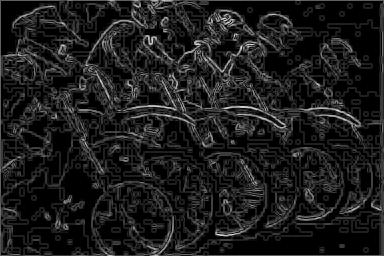
\includegraphics[width=\textwidth]{./figs/jpeg_mag}
         \caption{gradient magnitude of the Jpeg-compressed image}
         \label{fig:gmsd_jpeg_mag}
     \end{subfigure}
     \hfill
     \begin{subfigure}[b]{0.3\textwidth}
         \centering
         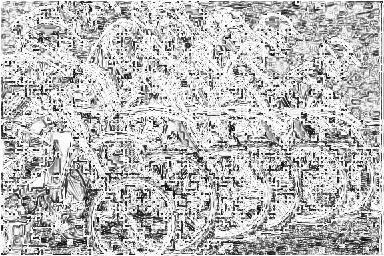
\includegraphics[width=\textwidth]{./figs/jpeg_sim}
         \caption{gradient magnitude similarity of the Jpeg image}
         \label{fig:gmsd_jpeg_sim}
     \end{subfigure}
     \\
     \begin{subfigure}[b]{0.3\textwidth}
         \centering
         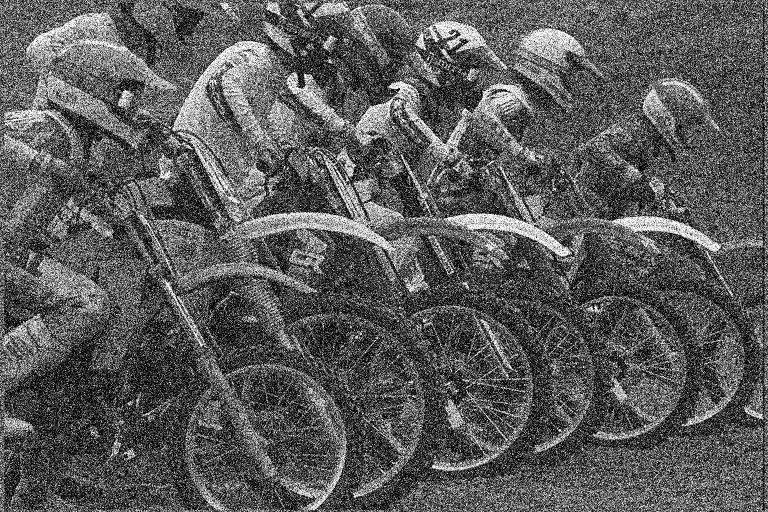
\includegraphics[width=\textwidth]{./figs/noise_gry}
         \caption{noisy image\\.}
         \label{fig:gmsd_noise_gry}
     \end{subfigure}
     \hfill
     \begin{subfigure}[b]{0.3\textwidth}
         \centering
         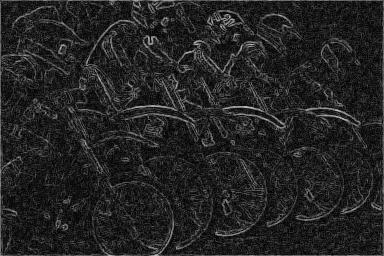
\includegraphics[width=\textwidth]{./figs/noise_mag}
         \caption{gradient magnitude of the noisy image}
         \label{fig:gmsd_noise_mag}
     \end{subfigure}
     \hfill
     \begin{subfigure}[b]{0.3\textwidth}
         \centering
         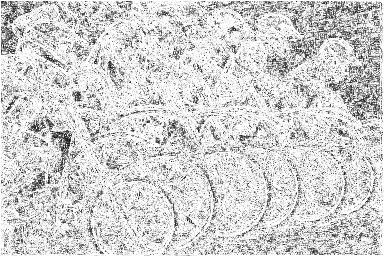
\includegraphics[width=\textwidth]{./figs/noise_sim}
         \caption{gradient magnitude similariy of the noisy image}
         \label{fig:gmsd_noise_sim}
     \end{subfigure}
        \caption{Different versions of an image with different distortions along with the gradient magnitude map and the map of gradient magnitude similarity with the original image.}
        \label{fig:gmsd}
\end{figure}
In Fig.~\ref{fig:gmsd} a sample is illustrated with its distorted versions and their gradient magnitudes. It is observable that image edges are sensitive to distortions. \underline{G}radient \underline{m}agnitude \underline{s}imilarity map for $r$ and $d$ is called $GMS(r, d)$ and defined as:
\begin{equation}
    GMS(r, d)_{(x, y)} = sim\left(GM_r(x, y), GM_d(x, y), c\right)
    \label{eq:gms}
\end{equation}
It is seen in Fig.~\ref{fig:gmsd_ref_sim} that GMS of an image and itself, equals to one for all pixels and when the image is degraded, this value will decrease (images in the right column).

GMSD computes the standard \underline{d}eviation for pooling the values of GMS. If $GMS(r, d)$ has $N$ pixels and $GMS(r, d)_x$ is the $x^{th}$ pixel, $GMSD(r, d)$ is obtained from the following equation:
\begin{equation}
    GMSD(r, d) = \sqrt{\frac{1}{N-1}\sum_{x=1}^{N}\left(GMS(r, d)_x-\frac{1}{N}\sum_{x=1}^NGMS(r, d)_x\right)^2}
\end{equation}
GMSD could improve the performance of SSIM, meanwhile, maintain a low computational complexity.

Considering image entropy~\cite{Sheikh2005, Sheikh2006}, different pooling strategies~\cite{Zhang2014a}, using image singular values~\cite{Mansouri2009, Mansouri2019}, analysis in wavelet domain~\cite{Chandler2007}, and taking color into account~\cite{Zhang2011a}, have been other innovations for FR IQA of singly distorted images.
%------------------------------------------------------------------------------------
\section{No-Reference IQA Methods}
%------------------------------------------------------------------------------------
The common approach of FR metrics is to define the quality score using mathematical relations~\cite{lin2010perceptual}. In the NR scenario, the distorted image is usually described with a feature vector and a model maps the vector to a quality score. This model can be a mathematical relation or be obtained using machine learning. The challenge for many NR IQA algorithms is to devise features that are expressive and fast to compute. Another strategy for feature extraction, is the use of machine learning techniques, such as \emph{convolutional neural networks-CNNs}. With CNNs, the feature vector can be achieved automatically. In what follows, the framework of \emph{feature-based} methods is presented, then the methods that are based on automatic feature extraction are reviewed.
\subsection{Feature-Based NR IQA Methods}
A common scheme for NR assessment, is extracting quality-relevant features. Then, with the use of machine learning methods, such as~\emph{support vector regression-SVR}, the features are mapped to quality scores. The required training data for machine learning can be obtained from the subjective scores in the image quality databases. The performance of these methods is dependent on the ability of the features to express the quality aspects of the image. The frameworks for training and testing of these methods is illustrated in Fig.~\ref{fig:svr_train} and Fig.~\ref{fig:svr_test}.
\begin{figure}
    \centering
    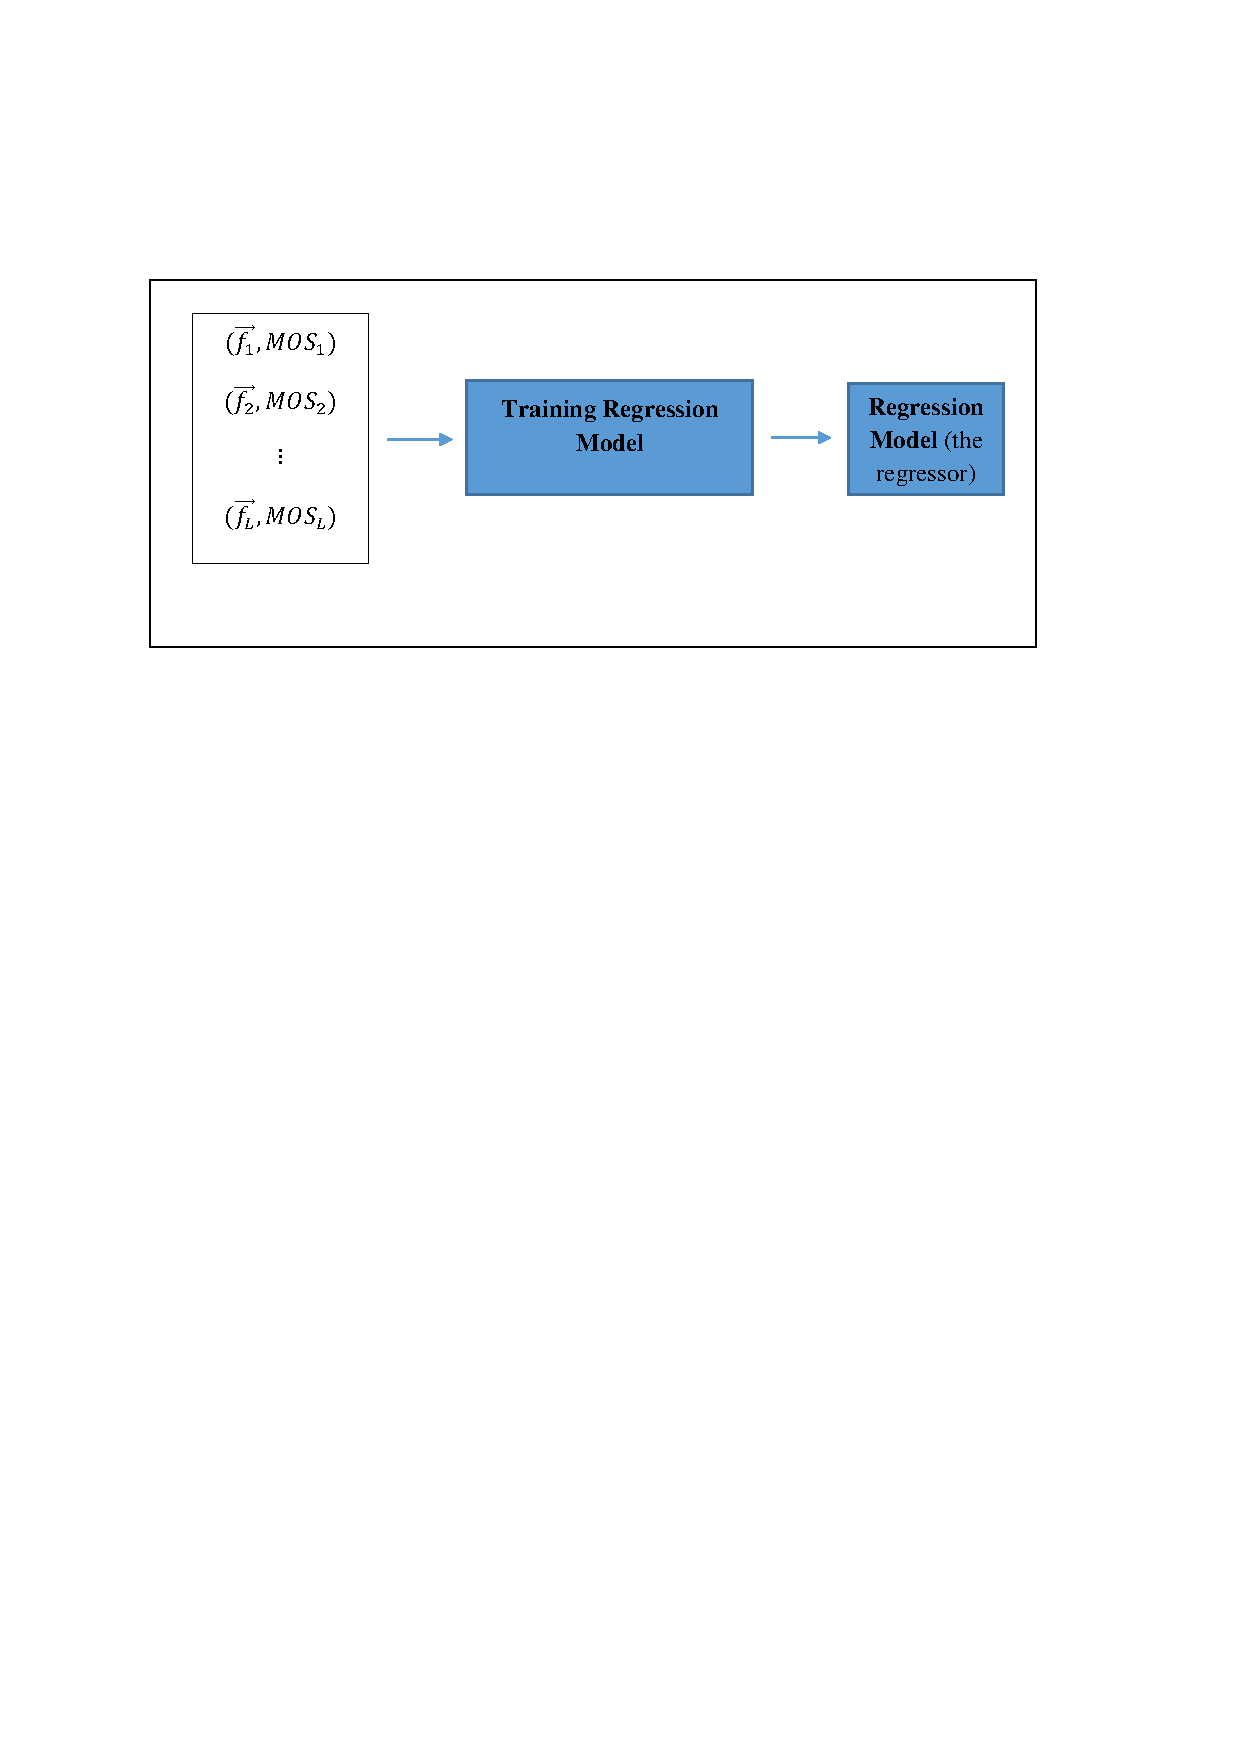
\includegraphics[width=\textwidth, trim={2.5cm 18.7cm 3.4cm 4.7cm}, clip]{./figs/fg_svr_train}
    \caption{Training feature-based methods}
    \label{fig:svr_train}
\end{figure}

\begin{figure}
    \centering
    \fbox{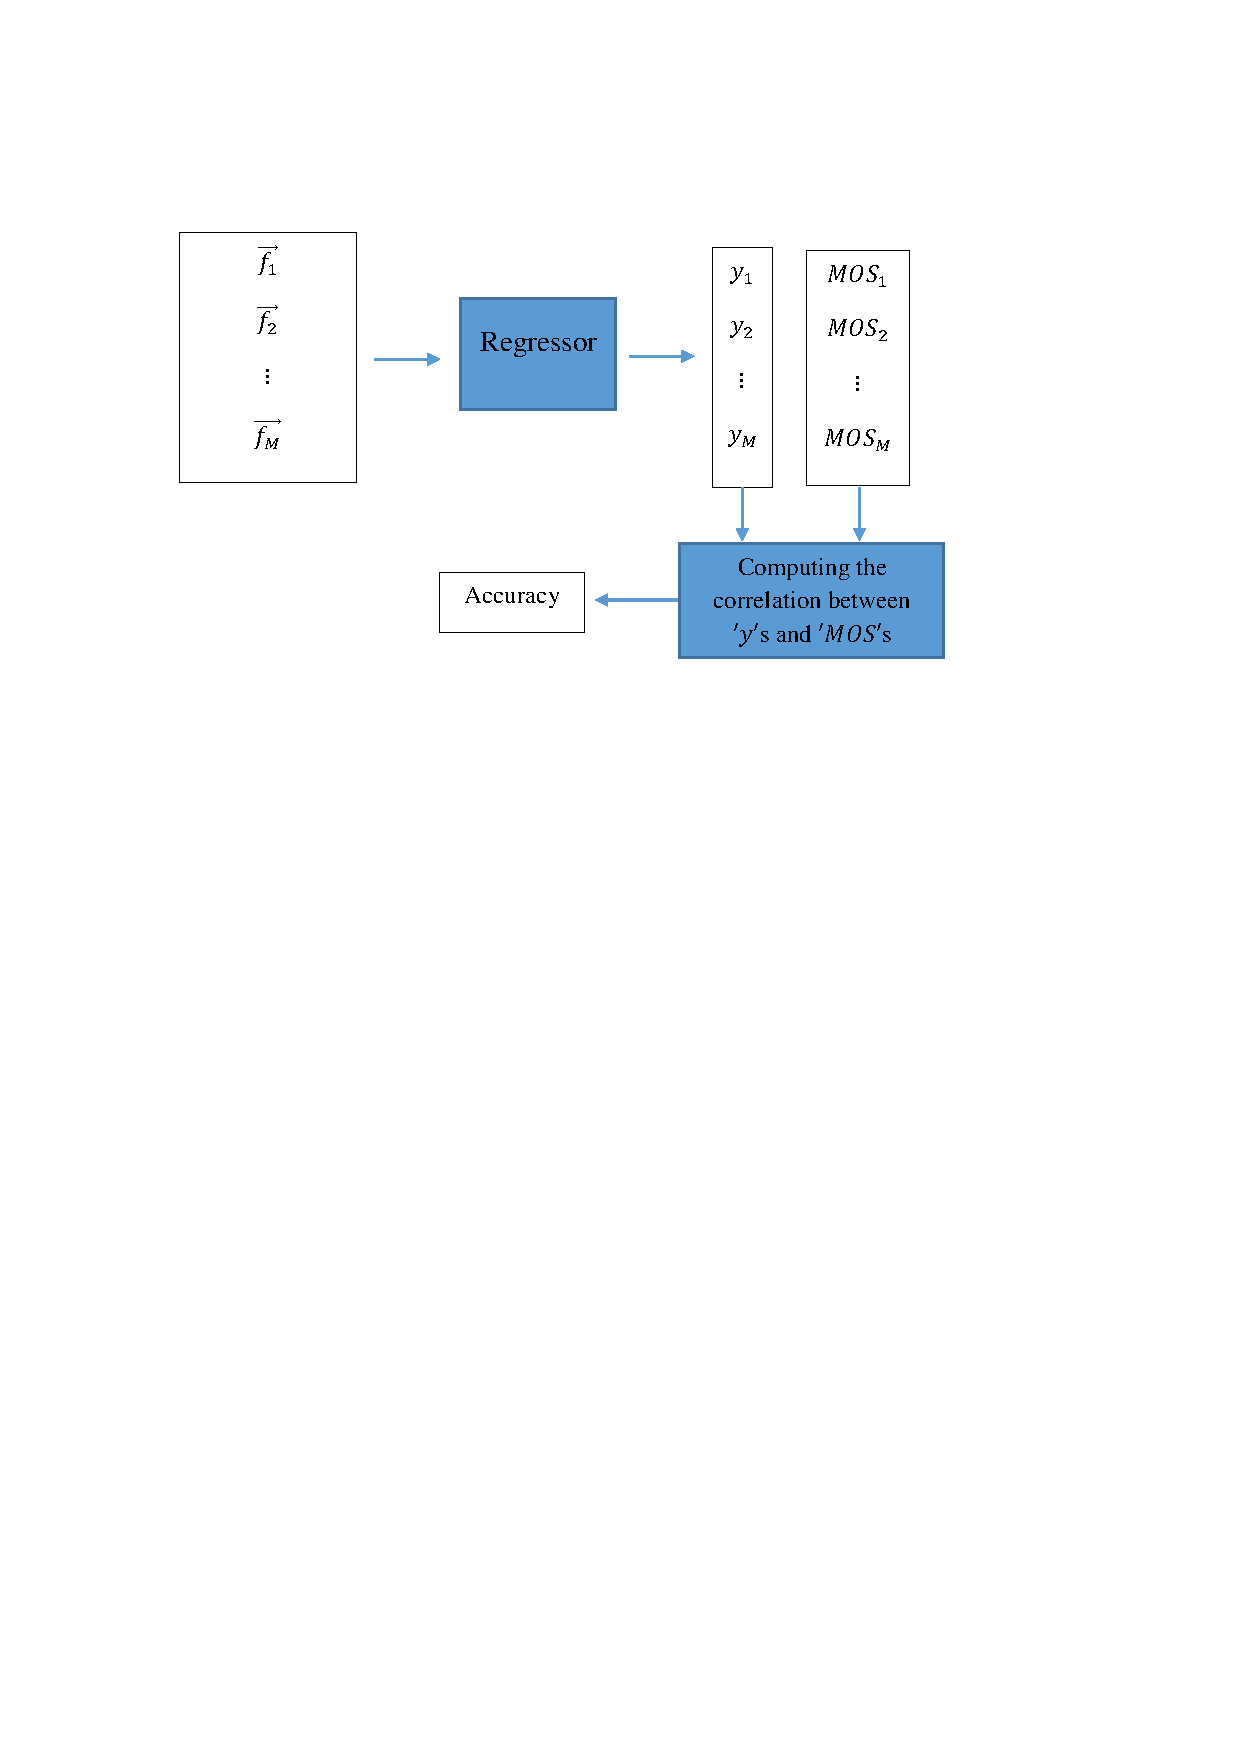
\includegraphics[width=0.97\textwidth, trim={2.8cm 18.3cm 4.8cm 3.8cm}, clip]{./figs/fg_svr_test}}
    \caption{Testing feature-based methods (The `Regressor' is the output of the train process.)}
    \label{fig:svr_test}
\end{figure}
If a dataset contains $N$ pictures and their corresponding human scores, it can be considered as a set of ordered pairs like $(I_i, MOS_i)$, where $I_i$ is the $i^{th}$ image and $MOS_i$ is the subjective score of $I_i$ for $i\in\{1,2,\ldots, N\}$. These ordered pairs are the `samples'. If a feature vector is extracted from $I_i$ it will be named: $\Vec{f}_i$. If $L$ samples of the dataset are selected for train, and, $M$ samples for test, a model can be trained on $L$ samples (Fig.~\ref{fig:svr_train}) and tested on the other $M$ samples (Fig.\ref{fig:svr_test}). It must be noted that $L+M=N$. The more the scores of the model are correlated with $MOS$s, the better is the performance of the method. The learning model in this framework can be a SVR~\cite{Vapnik1995} or a neural network. Although this model is effective in method's performance, but the main contribution to accuracy and speed, is made by the feature extraction mechanism.

Natural scene statistics is a common criterion for extracting features. Consider the two pictures in Fig.~\ref{fig:mscnhst} of `bikes' and `monarch' butterfly. If these images are transformed to MSCN\footnote{Calculation of the \emph{Mean-Subtracted \& Contrast-Normalized} image will be explained in the following paragraphs.} domain, their frequency histogram will obey the normal distribution (Fig.~\ref{fig:mscnhst_hst_bikes} and Fig.~\ref{fig:mscnhst_hst_monarch}). Ruderman~\cite{Ruderman1994} demonstrated that this distribution will be normal for any natural image, regardless of its content. If an image is distorted, it deviates from the natural state and it is expected that its distribution in the MSCN domain deviates from the normal distribution.
\begin{figure}
     \centering
     \begin{subfigure}[b]{0.3\textwidth}
         \centering
         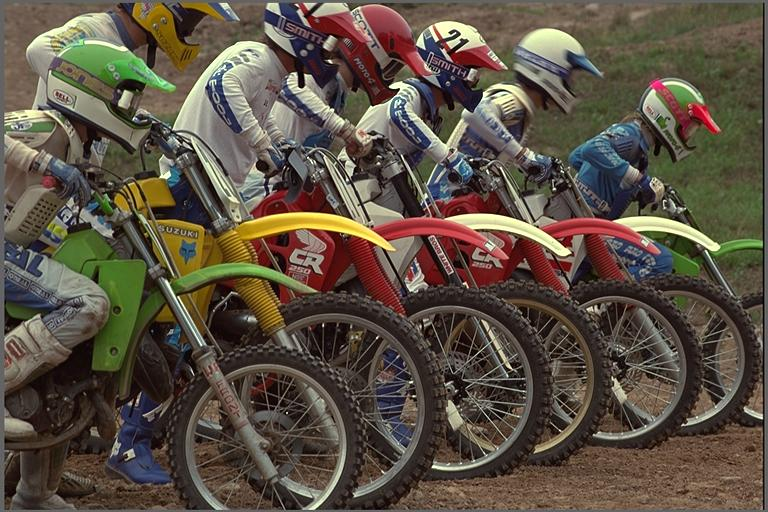
\includegraphics[width=\textwidth]{./figs/reference}
         \caption{`bikes'}
         \label{fig:mscnhst_bikes}
     \end{subfigure}
     \hfill
     \begin{subfigure}[b]{0.3\textwidth}
         \centering
         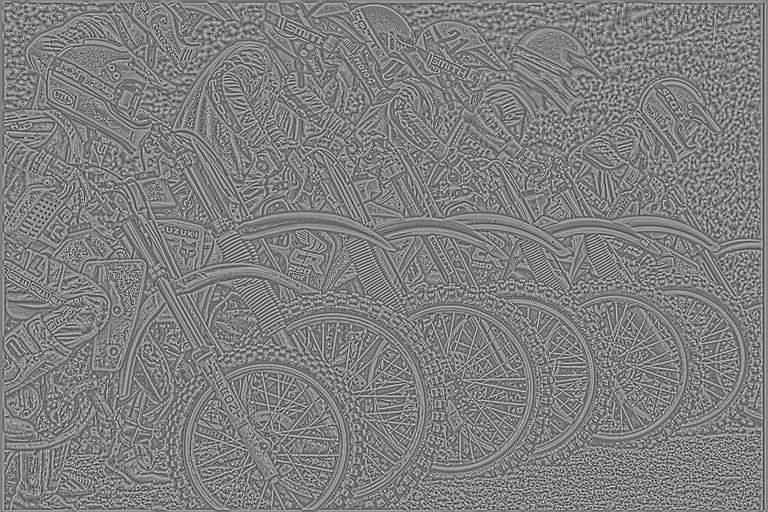
\includegraphics[width=\textwidth]{./figs/mscn_reference}
         \caption{MSCN version of `bikes'}
         \label{fig:mscnhst_mscn_bikes}
     \end{subfigure}
     \hfill
     \begin{subfigure}[b]{0.3\textwidth}
         \centering
         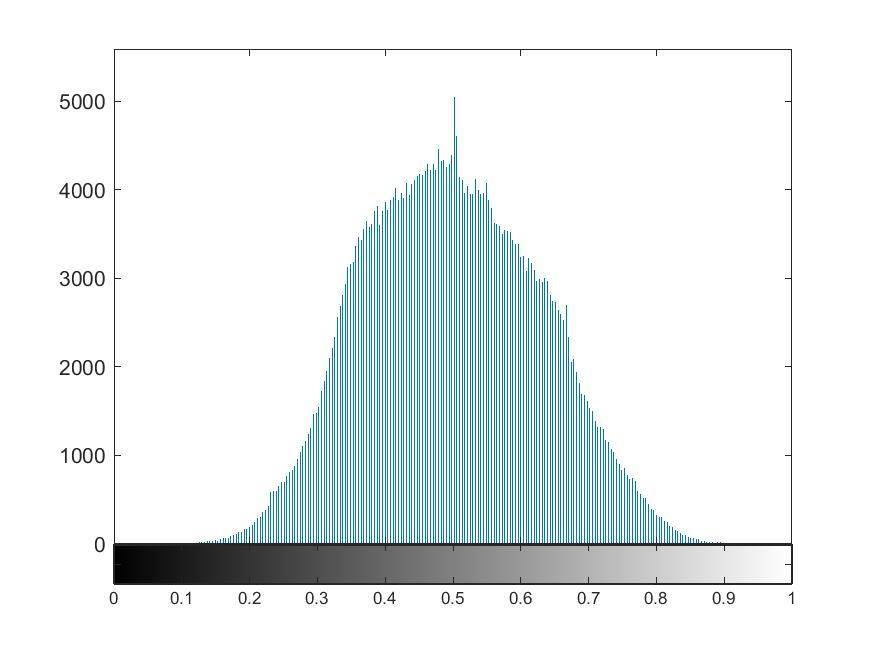
\includegraphics[width=\textwidth]{./figs/mscn_histreference}
         \caption{histogram of MSCN map}
         \label{fig:mscnhst_hst_bikes}
     \end{subfigure}
     \\
     \begin{subfigure}[b]{0.3\textwidth}
         \centering
         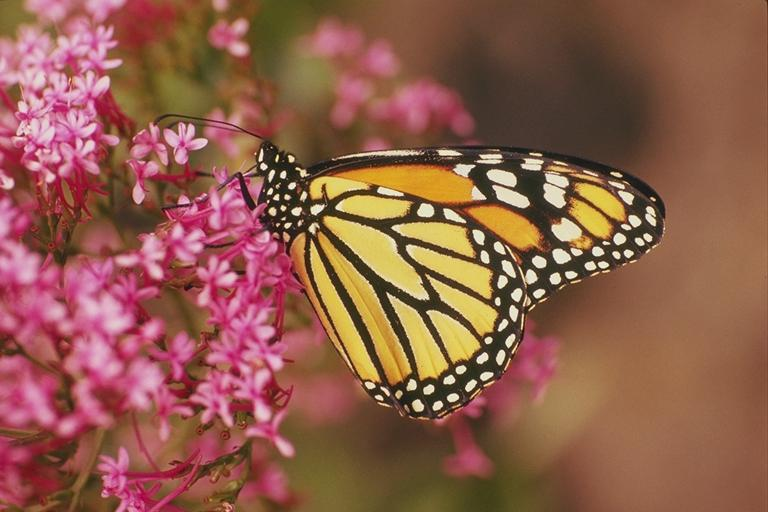
\includegraphics[width=\textwidth]{./figs/monarch}
         \caption{`monarch'}
         \label{fig:mscnhst_monarch}
     \end{subfigure}
     \hfill
     \begin{subfigure}[b]{0.3\textwidth}
         \centering
         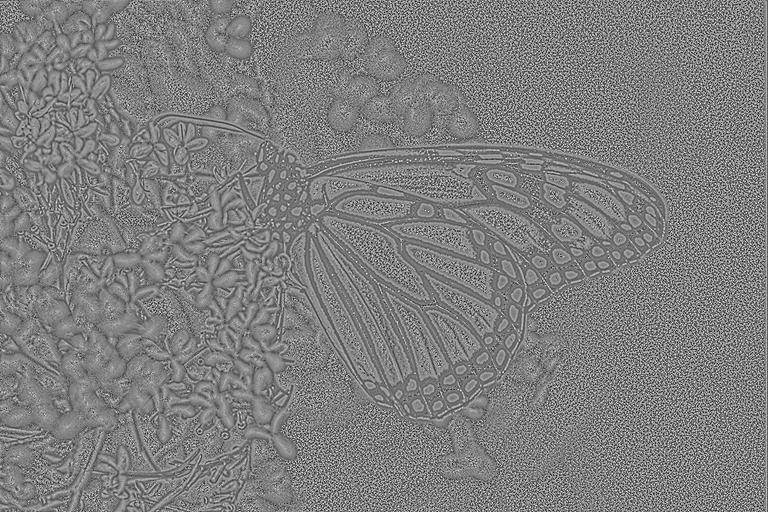
\includegraphics[width=\textwidth]{./figs/mscn_monarch}
         \caption{MSCN map of `monarch'}
         \label{fig:mscnhst_mscn_monarch}
     \end{subfigure}
     \hfill
     \begin{subfigure}[b]{0.3\textwidth}
         \centering
         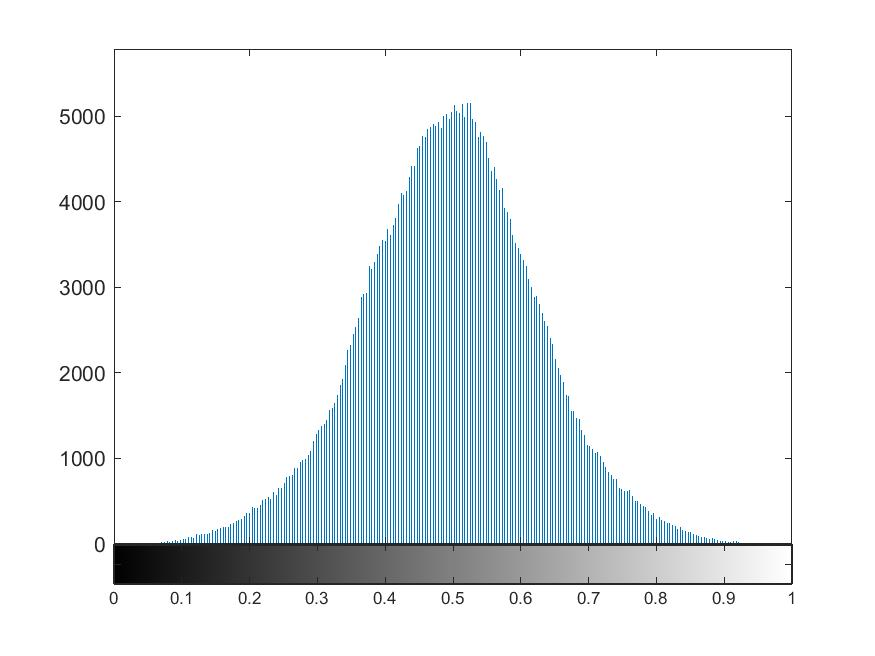
\includegraphics[width=\textwidth]{./figs/mscn_histmonarch}
         \caption{histogram of MSCN map}
         \label{fig:mscnhst_hst_monarch}
     \end{subfigure}
        \caption{Two images from LIVE dataset and their MSCN map and the histogram of values in the MSCN domain}
        \label{fig:mscnhst}
\end{figure}
In Fig~\ref{fig:nss} the histogram of MSCN maps are shown for the distorted versions of `bikes' and `monarch'. It is seen that despite the different contents of the two images, the distributions change with respect to type, and intensity of the distortions. For example, the Jpeg histogram has the same shape for both scenes (Fig.~\ref{fig:nss10} and Fi.g~\ref{fig:nss11}). Therefore, the MSCN distribution of a picture can be used to detect distortion.
\begin{figure}
     \centering
     \begin{subfigure}[b]{0.23\textwidth}
         \centering
         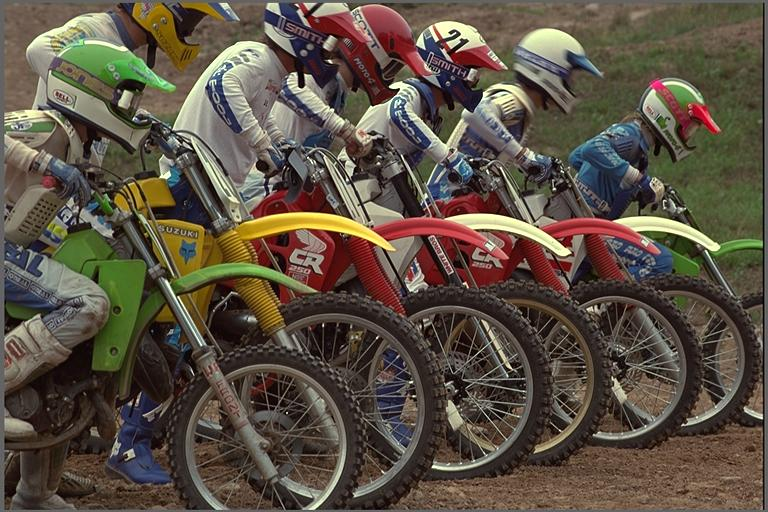
\includegraphics[width=\textwidth]{./figs/reference}
         \caption{}
         \label{fig:nss1}
     \end{subfigure}
     %\hfill
     \begin{subfigure}[b]{0.23\textwidth}
         \centering
         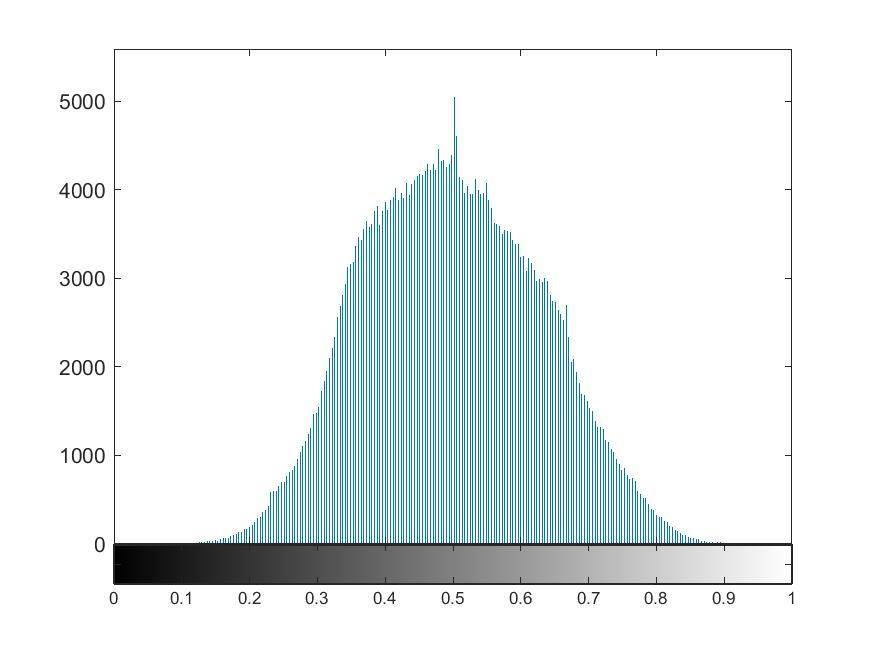
\includegraphics[width=\textwidth]{./figs/mscn_histreference}
         \caption{}
         \label{fig:nss2}
     \end{subfigure}
     %\hfill
     \begin{subfigure}[b]{0.23\textwidth}
         \centering
         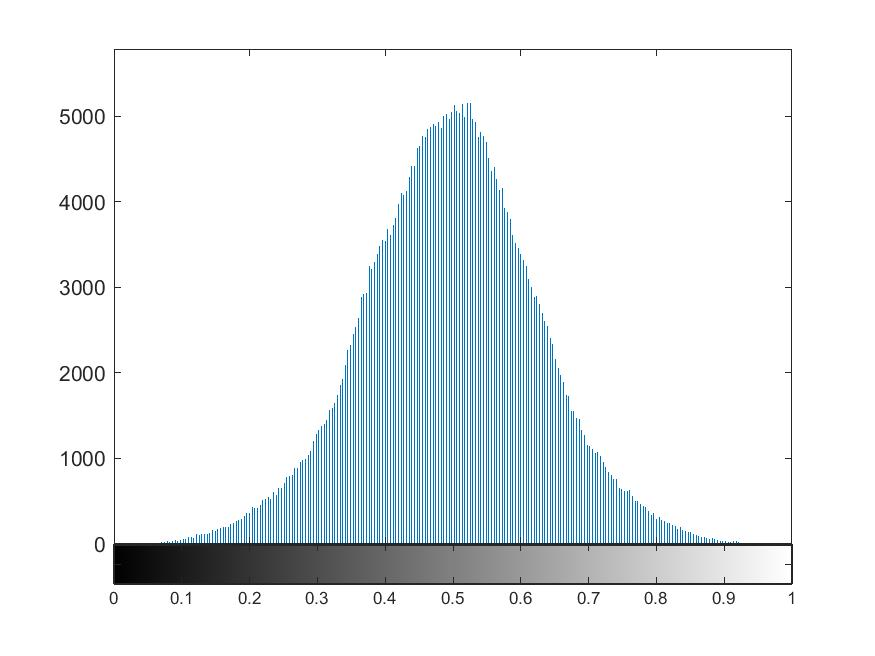
\includegraphics[width=\textwidth]{./figs/mscn_histmonarch}
         \caption{}
         \label{fig:nss3}
     \end{subfigure}
     \begin{subfigure}[b]{0.23\textwidth}
         \centering
         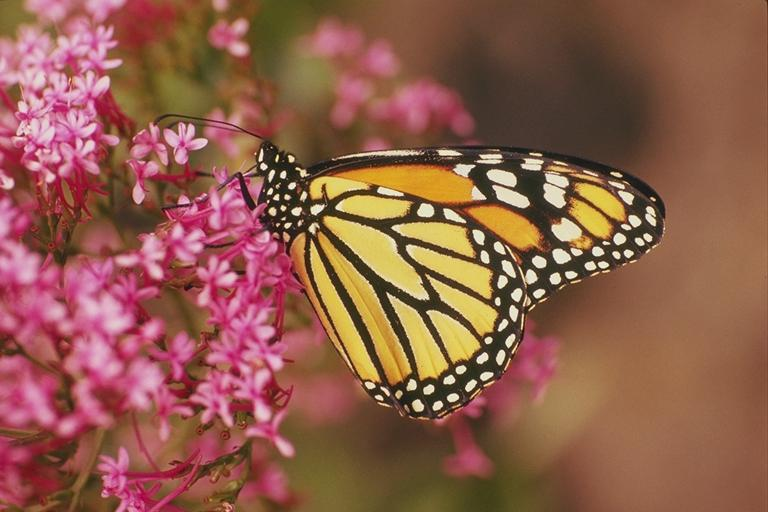
\includegraphics[width=\textwidth]{./figs/monarch}
         \caption{}
         \label{fig:nss4}
     \end{subfigure}
     \\
     \begin{subfigure}[b]{0.23\textwidth}
         \centering
         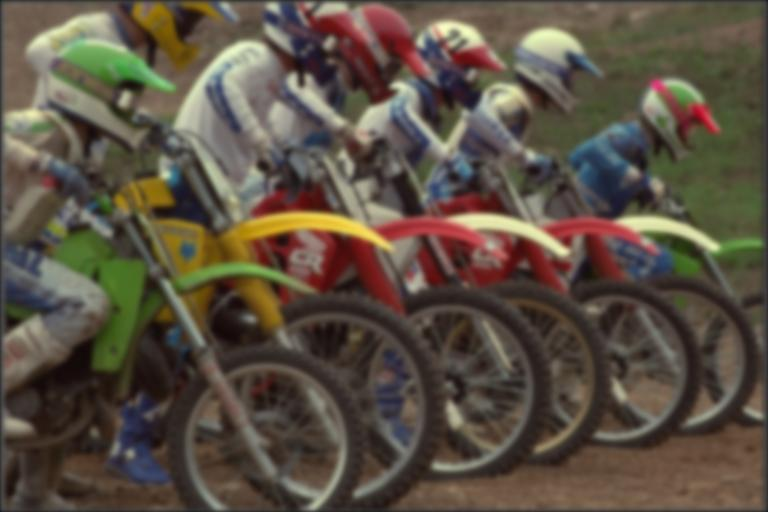
\includegraphics[width=\textwidth]{./figs/blur}
         \caption{}
         \label{fig:nss5}
     \end{subfigure}
     %\hfill
     \begin{subfigure}[b]{0.23\textwidth}
         \centering
         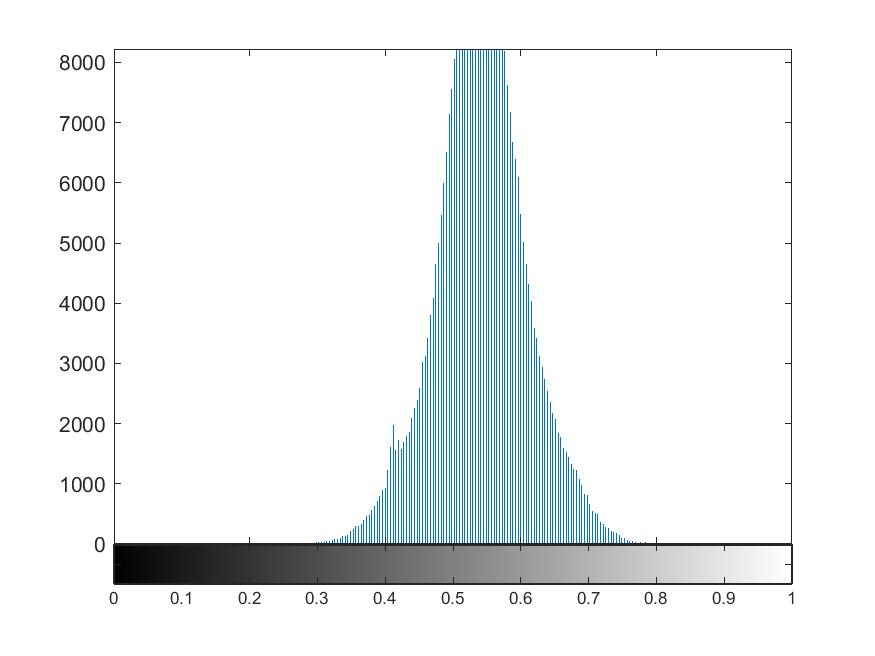
\includegraphics[width=\textwidth]{./figs/mscn_histblur}
         \caption{}
         \label{fig:nss6}
     \end{subfigure}
     %\hfill
     \begin{subfigure}[b]{0.23\textwidth}
         \centering
         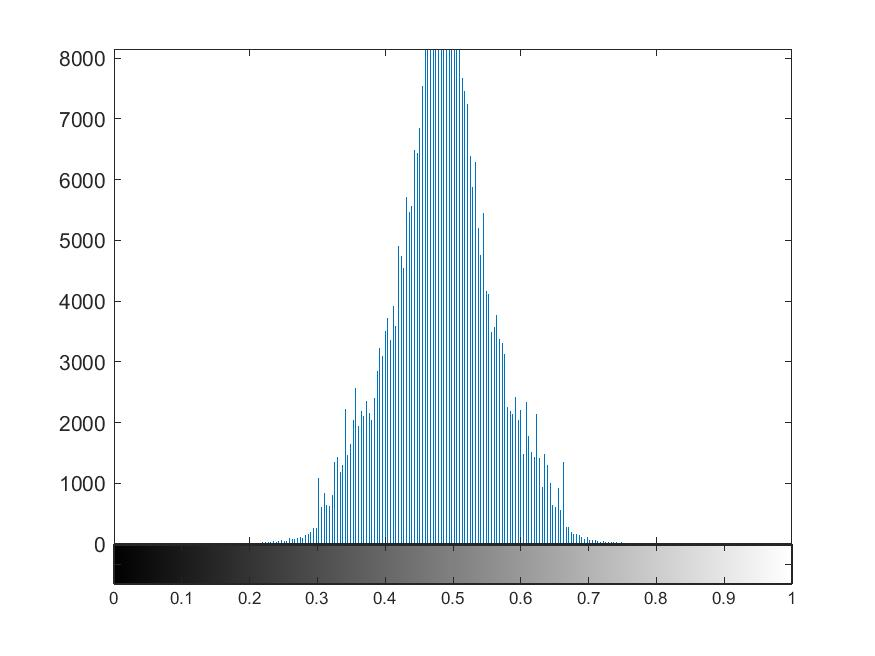
\includegraphics[width=\textwidth]{./figs/mscn_histmblur}
         \caption{}
         \label{fig:nss7}
     \end{subfigure}
     \begin{subfigure}[b]{0.23\textwidth}
         \centering
         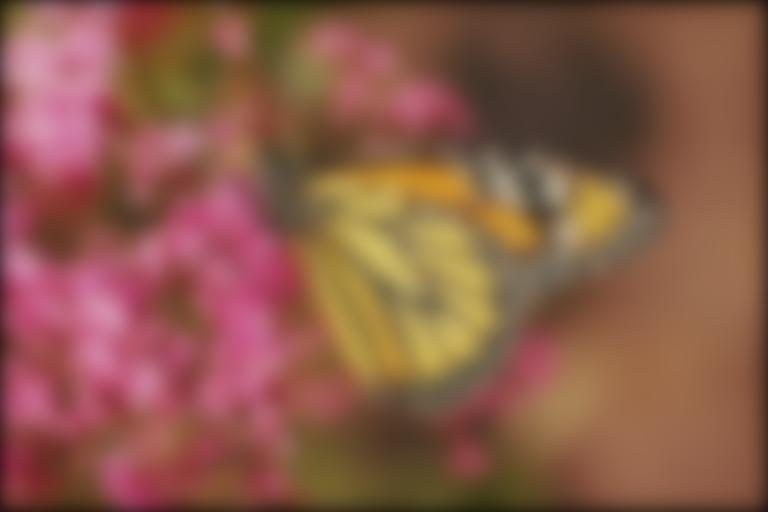
\includegraphics[width=\textwidth]{./figs/mblur}
         \caption{}
         \label{fig:nss8}
     \end{subfigure}
     \\
     \begin{subfigure}[b]{0.23\textwidth}
         \centering
         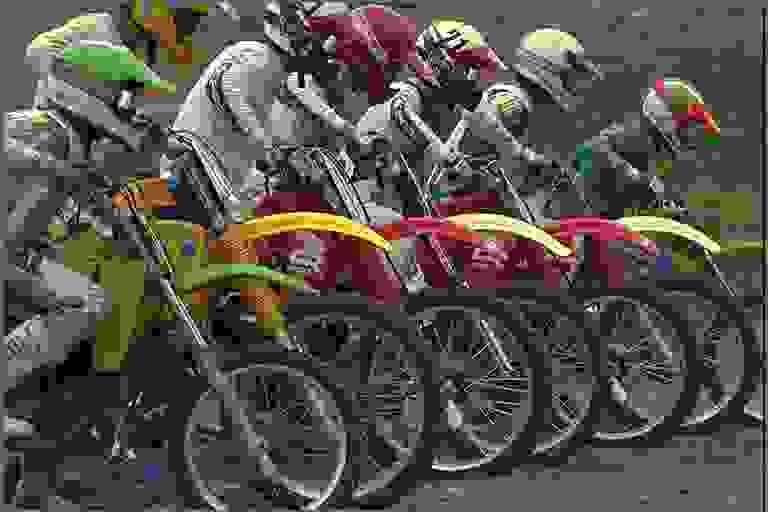
\includegraphics[width=\textwidth]{./figs/jpeg}
         \caption{}
         \label{fig:nss9}
     \end{subfigure}
     %\hfill
     \begin{subfigure}[b]{0.23\textwidth}
         \centering
         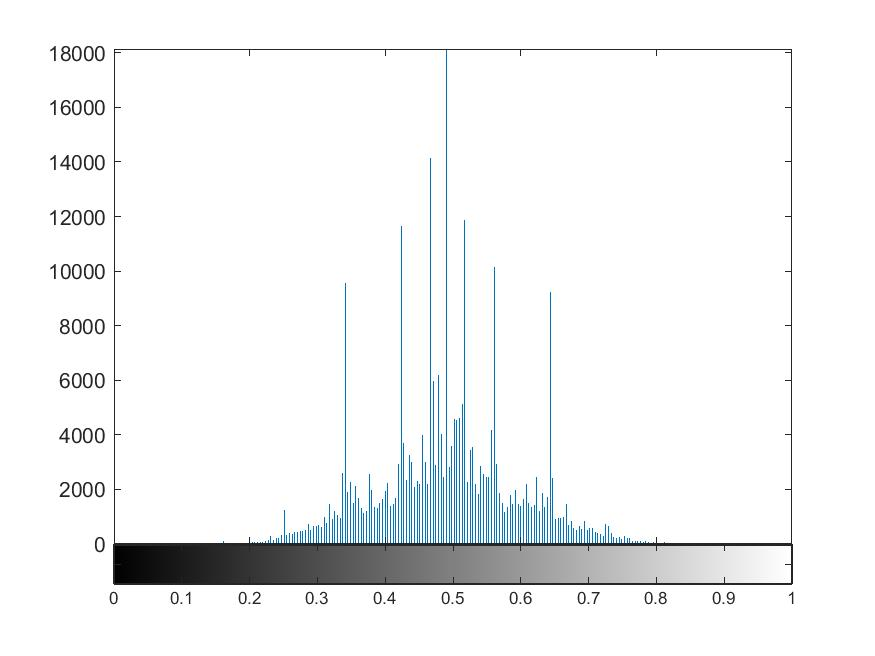
\includegraphics[width=\textwidth]{./figs/mscn_histjpeg}
         \caption{}
         \label{fig:nss10}
     \end{subfigure}
     %\hfill
     \begin{subfigure}[b]{0.23\textwidth}
         \centering
         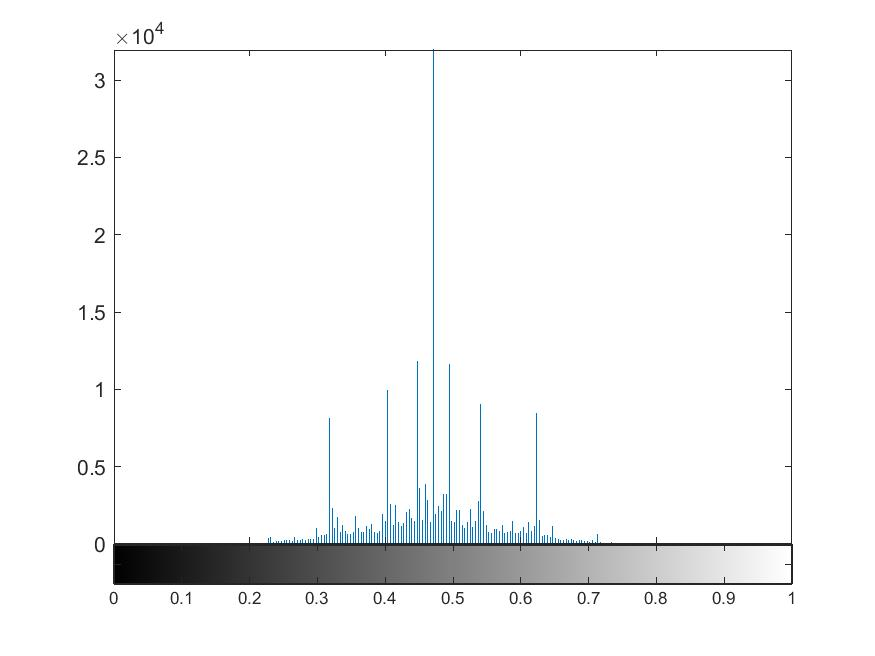
\includegraphics[width=\textwidth]{./figs/mscn_histmjpeg}
         \caption{}
         \label{fig:nss11}
     \end{subfigure}
     \begin{subfigure}[b]{0.23\textwidth}
         \centering
         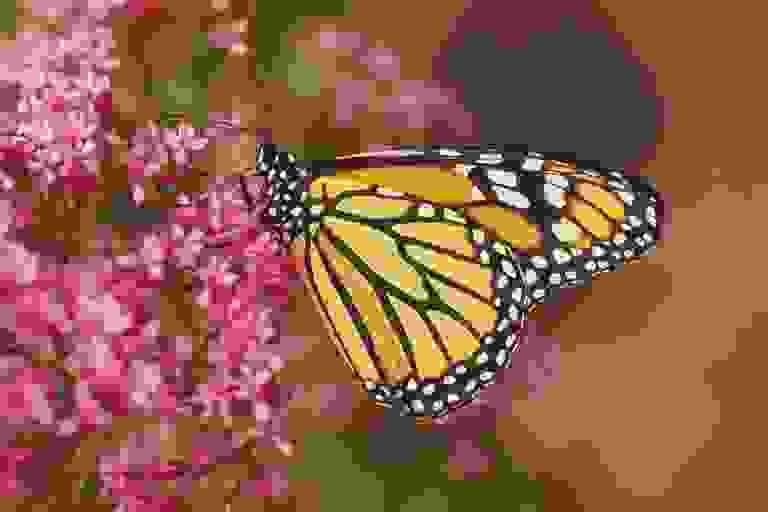
\includegraphics[width=\textwidth]{./figs/mjpeg}
         \caption{}
         \label{fig:nss12}
     \end{subfigure}
     \\
     \begin{subfigure}[b]{0.23\textwidth}
         \centering
         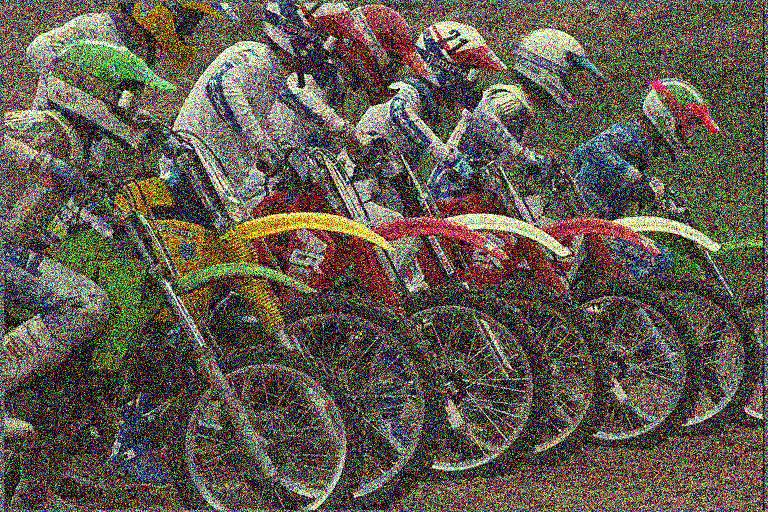
\includegraphics[width=\textwidth]{./figs/noise}
         \caption{}
         \label{fig:nss13}
     \end{subfigure}
     %\hfill
     \begin{subfigure}[b]{0.23\textwidth}
         \centering
         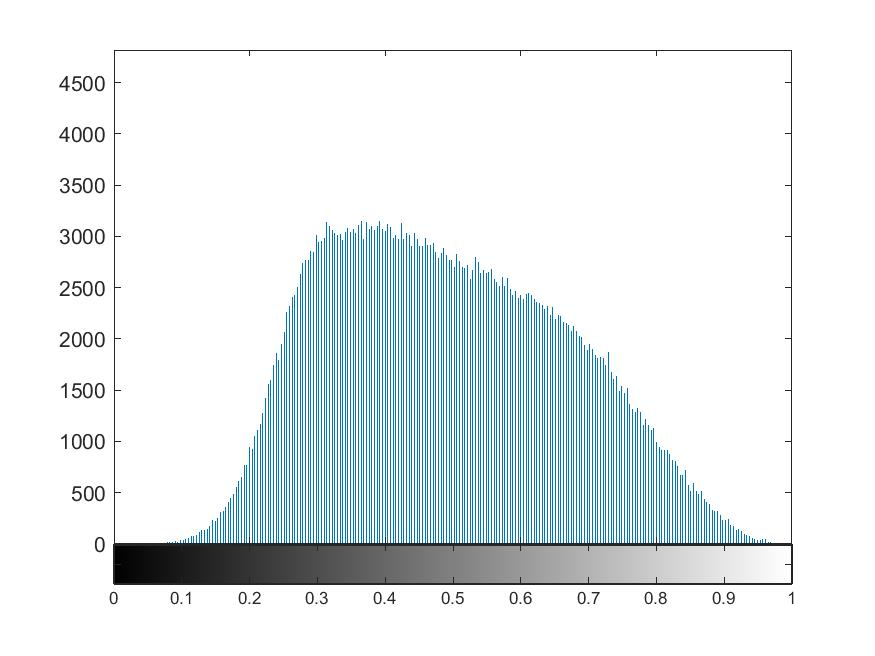
\includegraphics[width=\textwidth]{./figs/mscn_histnoise}
         \caption{}
         \label{fig:nss14}
     \end{subfigure}
     %\hfill
     \begin{subfigure}[b]{0.23\textwidth}
         \centering
         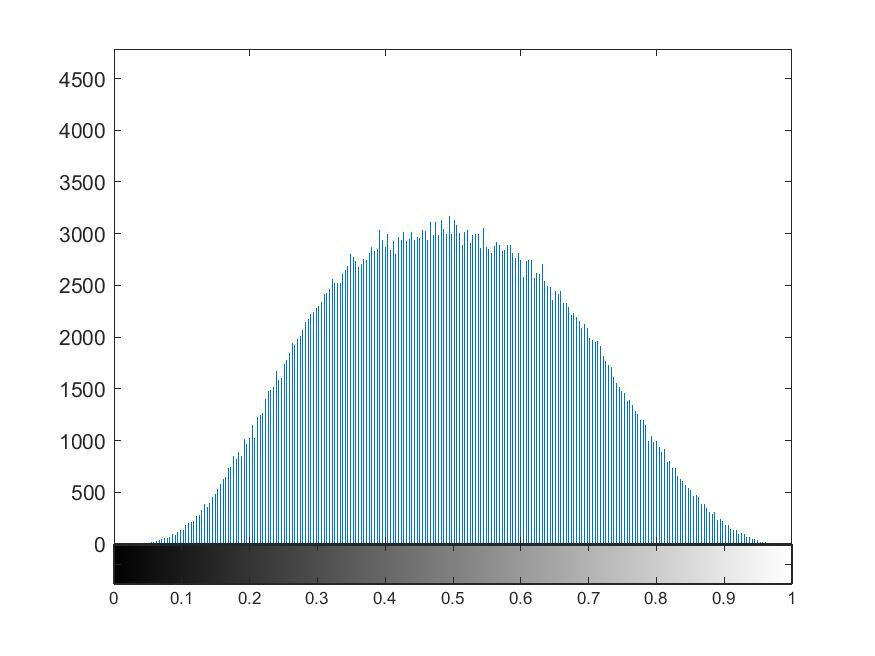
\includegraphics[width=\textwidth]{./figs/mscn_histmnoise}
         \caption{}
         \label{fig:nss15}
     \end{subfigure}
     \begin{subfigure}[b]{0.23\textwidth}
         \centering
         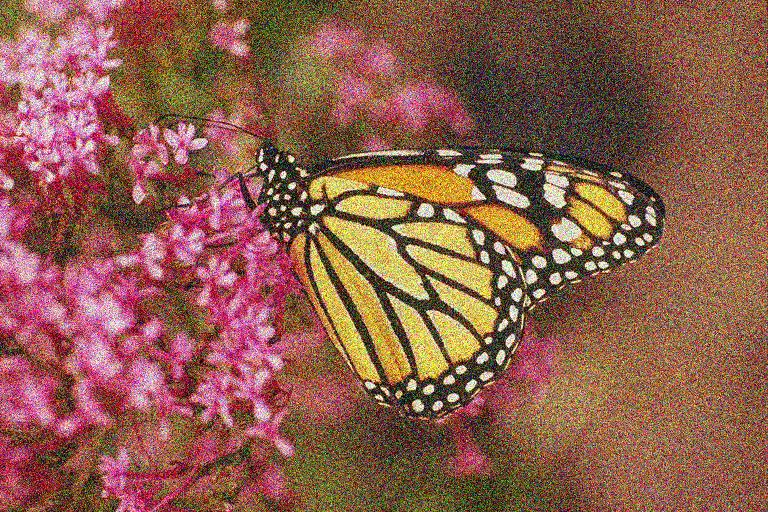
\includegraphics[width=\textwidth]{./figs/mnoise}
         \caption{}
         \label{fig:nss16}
     \end{subfigure}
        \caption{MSCN distributions for distorted versions of two images}
        \label{fig:nss}
\end{figure}
The MSCN value of the pixel at $(x, y)$ of the grayscale image $I$ is represented with $\hat{I}(x, y)$ and obtained from the following relation~\cite{Mittal2012a}:
\begin{equation}
    \hat{I}(x, y) = \frac{I(x, y)-\mu}{\sigma}
    \label{eq:mscn}
\end{equation}
Where $\mu$ and $\sigma$ are the mean and variance in a $3\times3$ neighborhood of $I(x, y)$. 

The distribution of MSCN values can also be fitted with a generalized Gaussian distribution (GGD)~\cite{sharifi1995estimation}. GGD has parameters, such as mean ($m$), variance ($\sigma$), and shape ($\alpha$). The estimated parameters for an image, can be considered as the elements of a feature vector that describes the quality of the image.

In fact, this is what the method BRISQUE~\cite{Mittal2012a} does. Beside MSCN coefficients, NSS of other domains have been explored. BIQI~\cite{Moorthy2010} uses NSS in wavelet domain and BLIINDS-II~\cite{Saad2012} computes the features based on the entropy and average of coefficients of discrete cosine transform (DCT). Also, other distributions have been used for describing the histograms such as Gaussian scale mixtures (GSM)~\cite{Gupta2018}.
%---------------------------------------------
\subsection{Automatic Feature Extraction}
%---------------------------------------------
Convolutional neural networks can also extract feature vectors~\cite{Badrinarayanan2017}. The common architecture of these networks pools multiple 2D-feature maps after many convolutional layers to a 1D-vector. Then, fully connected layers of neurons classify or regress the vector. Methods like CNN~\cite{Kang2014}, MEON~\cite{Ma2017a}, DIQaM-NR~\cite{Bosse2018}, and Rank-IQA~\cite{liu2017rankiqa} are examples of such networks.

Using CNNs, the feature extraction process is embedded in the network and it is difficult to interpret the computed features. This is the same for dictionary-based methods~\cite{Jurie2005}. In these methods, such as CORNIA~\cite{Ye2012b}, HOSA~\cite{Xu2016}, QAF~\cite{Zhang2014}, SOM~\cite{Zhang2015b}, and QAC~\cite{Xue2013}, the distorted image is coded in a feature vector, based on a dictionary that contains the features of all good images. This dictionary is built by clustering the features of a set of good quality images.

Automatic features are shown to be expressive. In neural networks, these features are jointly optimized with the model that computes the scores, which increases the accuracy. However, the computational complexity of these methods is high and they demand large numbers of training samples. As mentioned earlier, these features are not interpretable and their relation with quality aspects of the image cannot be analyzed.
% --------------------------------------------
\section{FR methods for Multiple Distortions}
% --------------------------------------------
The existence of multiple distortions in an image, makes quality prediction difficult~\cite{Chandler2013}. Even if we can measure the severity of each distortion correctly, their \emph{joint effect} on the perceived quality will be difficult to predict, since their combination is not linear and depends on the type of distortions~\cite{goodman1979multidimensional}. The accurate measurement of distortions' intensity in the presence of other distortions, is also controversial~\cite{linde1981similarity} and necessitates to consider the \emph{mutual effect} of the distortions on each other. As an example, assume adding a fixed amount of noise to two images; a sharp image and its blurry version. Normally the noise will be more sensible in the blurry version. Similarly, it is expected that blurring a noisy image must alleviate the effect of noise~\cite{linde1981similarity}. However, subjective experiments~\cite{Kayargadde1996} show that this is true in some cases and completely wrong for many common samples.

These observations show the difficulty of assessing multiple distortions and reveal that accurate prediction of each combination or even permutation of distortions can be quite different. Thus, optimization for a specific permutation may result in poor performance for others. Some of methods for multiple distortions, tried to estimate or model the joint and mutual effect of the distortions. In the rest of the section, different methods for IQA of multiply-distorted images are reviewed and analyzed.
% --------------------------------
\subsection{Combination of Scores}
% --------------------------------
Combining the scores of four singly-distorted metrics, was the solution for FR IQA of multiple distortions, proposed by Chetouani~\cite{Chetouani2016}. In this method, four scores are computed for the distorted image with methods VIF~\cite{Sheikh2006}, IFC~\cite{Sheikh2005}, WASH~\cite{Reenu2013}, and SSIM~\cite{Wang2004}. They are then fed to an SVR as a $1\times 4$ feature vector to be mapped to the quality score.

The four single distortion methods that are employed here, consider different criteria. SSIM measures structural similarity, VIF and IFC take images' entropy into account and WASH measures blurriness. With this combination, it has been tried to capture the effect of multiple distortions.

A similar approach was taken by Okarma in~\cite{Okarma2014} with the difference that a nonlinear combination of the scores was used to pool the scores of the single metrics to the final score. The coefficients and powers of this nonlinear combination were optimized using the subjective scores of multi-distortion IQA datasets.

Due to the difficulty of modeling the joint effect, Chetouani used SVR in order to let machine learning to estimate the correct combination based on the individual metrics. However, when using a trainable model, its ability to generalize to samples outside the training dataset must be tested as well. Meanwhile, FR methods are normally based on mathematical relation and compute the quality directly.

Another issue is that the methods in~\cite{Chetouani2016} and~\cite{Okarma2014} need to execute multiple independent metrics which is a huge computational load. This makes them very slow in comparison to the conventional FR metrics.
% -----------------------------------------------
\subsection{Similarity of QWT Subbands}
% ------------------------------------------------
Li et al.~\cite{Li2018a} used quaternion wavelet transform (QWT)~\cite{Muraleetharan2015} for extracting image structural information. At each scale, an image in QWT domain is decomposed into four subbands, $LL$, $LH$, $HL$, and $HH$. Each of these subbands has a magnitude, $M$, and three phases, $\theta$, $\phi$, and $\psi$ (Fig.~\ref{fig:qwt}).
\begin{figure}
     \centering
     \begin{subfigure}[b]{0.23\textwidth}
         \centering
         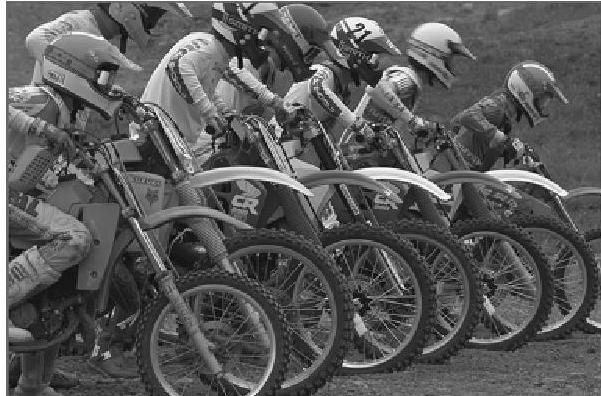
\includegraphics[width=\textwidth]{./figs/m_1_1_q}
         \caption{$LL_M$}
         \label{fig:qwt1}
     \end{subfigure}
     %\hfill
     \begin{subfigure}[b]{0.23\textwidth}
         \centering
         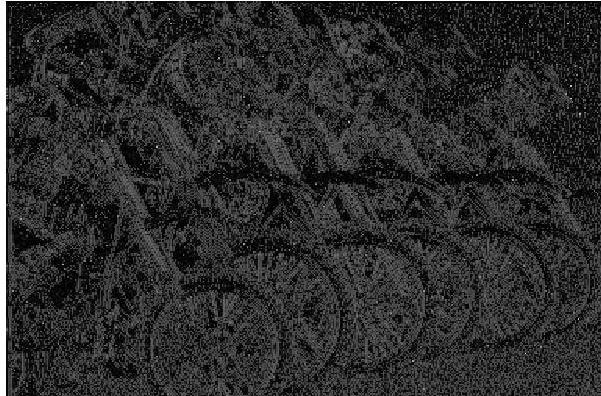
\includegraphics[width=\textwidth]{./figs/o_1_1_1_q}
         \caption{$LL_{\theta}$}
         \label{fig:qwt2}
     \end{subfigure}
     %\hfill
     \begin{subfigure}[b]{0.23\textwidth}
         \centering
         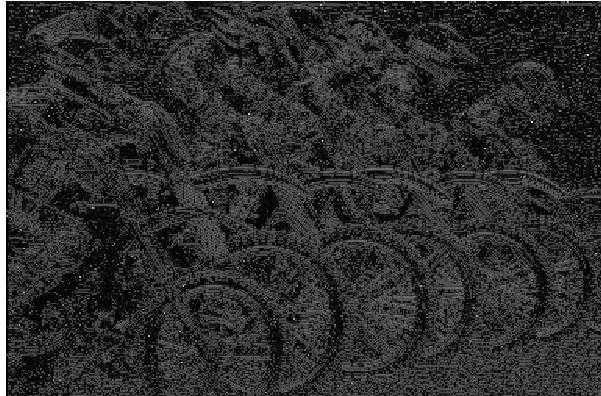
\includegraphics[width=\textwidth]{./figs/o_1_1_2_q}
         \caption{$LL_{\phi}$}
         \label{fig:qwt3}
     \end{subfigure}
     \begin{subfigure}[b]{0.23\textwidth}
         \centering
         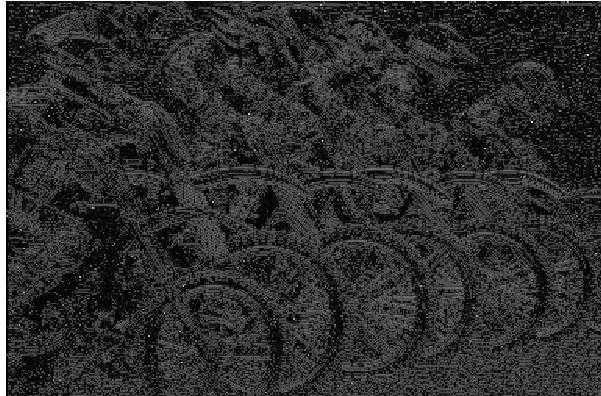
\includegraphics[width=\textwidth]{./figs/o_1_1_2_q}
         \caption{$LL_{\psi}$}
         \label{fig:qwt4}
     \end{subfigure}
     \\
     \begin{subfigure}[b]{0.23\textwidth}
         \centering
         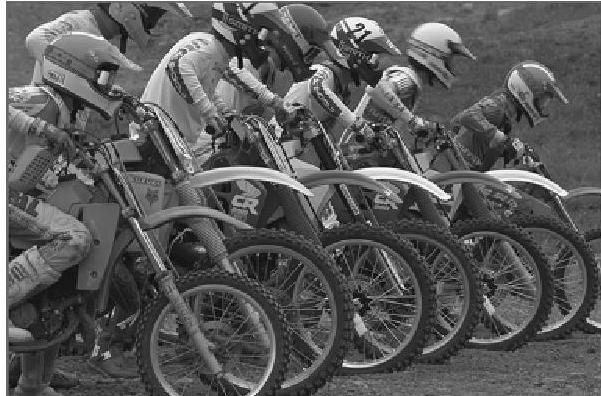
\includegraphics[width=\textwidth]{./figs/m_1_1_q}
         \caption{$LH_M$}
         \label{fig:qwt5}
     \end{subfigure}
     %\hfill
     \begin{subfigure}[b]{0.23\textwidth}
         \centering
         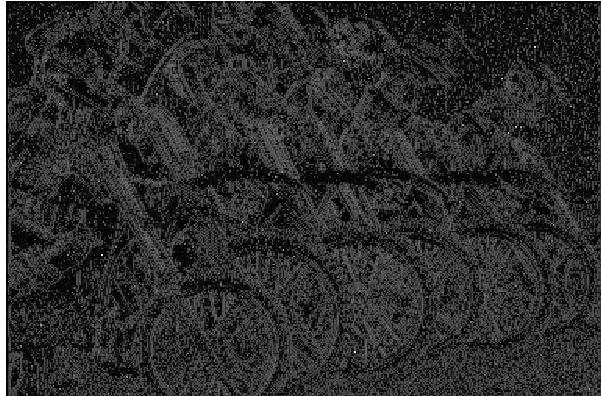
\includegraphics[width=\textwidth]{./figs/o_1_2_1_q}
         \caption{$LH_{\theta}$}
         \label{fig:qwt6}
     \end{subfigure}
     %\hfill
     \begin{subfigure}[b]{0.23\textwidth}
         \centering
         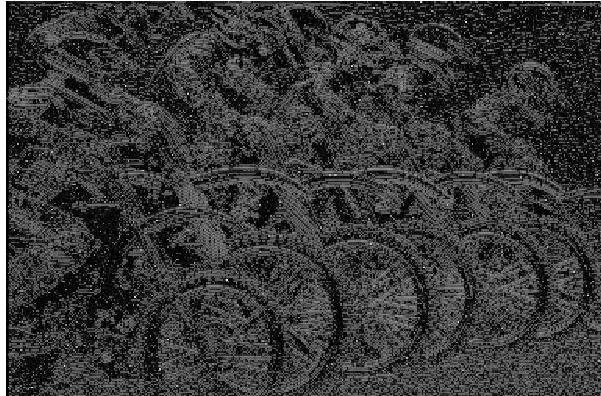
\includegraphics[width=\textwidth]{./figs/o_1_2_2_q}
         \caption{$LH_{\phi}$}
         \label{fig:qwt7}
     \end{subfigure}
     \begin{subfigure}[b]{0.23\textwidth}
         \centering
         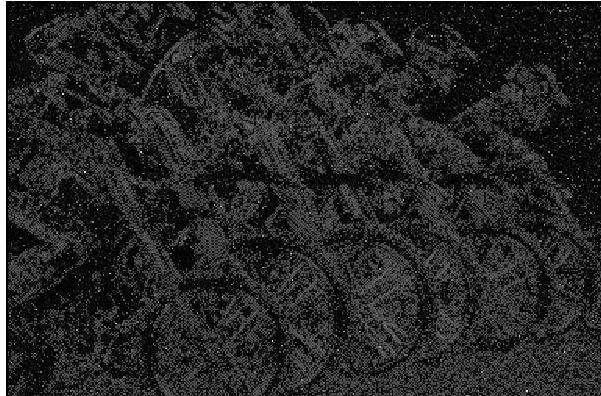
\includegraphics[width=\textwidth]{./figs/o_1_2_3_q}
         \caption{$LH_{\psi}$}
         \label{fig:qwt8}
     \end{subfigure}
     \\
     \begin{subfigure}[b]{0.23\textwidth}
         \centering
         \includegraphics[width=\textwidth]{./figs/m_2_1_q}
         \caption{$HL_M$}
         \label{fig:qwt9}
     \end{subfigure}
     %\hfill
     \begin{subfigure}[b]{0.23\textwidth}
         \centering
         \includegraphics[width=\textwidth]{./figs/o_2_1_1_q}
         \caption{$HL_{\theta}$}
         \label{fig:qwt10}
     \end{subfigure}
     %\hfill
     \begin{subfigure}[b]{0.23\textwidth}
         \centering
         \includegraphics[width=\textwidth]{./figs/o_2_1_2_q}
         \caption{$HL_{\phi}$}
         \label{fig:qwt11}
     \end{subfigure}
     \begin{subfigure}[b]{0.23\textwidth}
         \centering
         \includegraphics[width=\textwidth]{./figs/o_2_1_3_q}
         \caption{$HL_{\psi}$}
         \label{fig:qwt12}
     \end{subfigure}
     \\
     \begin{subfigure}[b]{0.23\textwidth}
         \centering
         \includegraphics[width=\textwidth]{./figs/m_2_2_q}
         \caption{$HH_M$}
         \label{fig:qwt13}
     \end{subfigure}
     %\hfill
     \begin{subfigure}[b]{0.23\textwidth}
         \centering
         \includegraphics[width=\textwidth]{./figs/o_2_2_1_q}
         \caption{$HH_{\theta}$}
         \label{fig:qwt14}
     \end{subfigure}
     %\hfill
     \begin{subfigure}[b]{0.23\textwidth}
         \centering
         \includegraphics[width=\textwidth]{./figs/o_2_2_2_q}
         \caption{$HH_{\phi}$}
         \label{fig:qwt15}
     \end{subfigure}
     \begin{subfigure}[b]{0.23\textwidth}
         \centering
         \includegraphics[width=\textwidth]{./figs/o_2_2_3_q}
         \caption{$HH_{\psi}$}
         \label{fig:qwt16}
     \end{subfigure}
        \caption{The QWT subbands of `bikes' in one scale}
        \label{fig:qwt}
\end{figure}
According to Fig.~\ref{fig:qwt}, subbands of QWT have fine characteristics for detecting distortions. The magnitude of $LL$, is an approximation of the entire image and roughly shift invariant. Phases of $LL$, demonstrate the horizontal, vertical and diagonal structures. The magnitudes of $LH$, $HL$, and $HH$, extract the edges in different directions. In their method, called QWT-IQA, Li et al. compare the magnitude and phases of subbands of the reference and distorted image. Then they compute the quality scores of each subband, which are named: $Q_{LL}$, $Q_{LH}$, $Q_{HL}$, and $Q_{HH}$.

The magnitude and phases are denoted as in Fig.~\ref{fig:qwt} and the corresponding terms in reference or distorted image, are distinguished with $R$ and $D$ subscripts. As an example, the computation of $Q_{LL}$ will be explained. To compare $LL_{M_R}$ and $LL_{M_D}$, their point-wise similarity will be calculated:
\begin{equation}
    LL_MS(x, y) = sim(LL_{M_D}(x, y), LL_{M_R}(x, y), c)
    \label{eq:LL_MS}
\end{equation}
$LL_MS$ is the similarity map of $LL_{M_D}$ and $LL_{M_R}$. Similarly, $LL_\theta S$, $LL_\phi S$, and $LL_\psi S$ can be calculated. To collapse the information in $LL_MS$, $LL_\theta S$, $LL_\phi S$, and $LL_\psi S$ into one map, their point-wise multiplication is calculated:
\begin{equation}
    LLS(x, y) = LL_MS^{10}(x, y)\times LL_\theta S(x, y)\times LL_\phi S(x, y)\times LL_\psi S(x, y)
    \label{eq:LLS}
\end{equation}
$LLS$ is the similarity map for the $LL$ subband of the reference and the distorted image. The power of $10$ for $LL_MS$ and $1$ for $LL_\theta S$, $LL_\phi S$, and $LL_\psi S$, is obtained experimentally. For pooling $LLS$ to one score, a weighted average of its values is computed. The weight of each pixel, $W(x, y)$, is the maximum of $LL_{M_R}$ and $LL_{M_D}$:
\begin{equation}
    W(x, y) = max\{LL_{M_R}(x, y), LL_{M_D}(x, y)\}
    \label{eq:weight_qwt}
\end{equation}
This weighting strategy is an effort to simulate an HVS property that relates to higher vision accuracy in brighter scenes~\cite{Gonzalez2008}. Pixels with larger values, correspond to brighter spots and contribute more in determining the quality score. The score of $LL$ is called $Q_{LL}$ and obtained from relation~\ref{eq:qwtiqa_LL}. The scores for other subbands can be computed similarly.
\begin{equation}
    Q_{LL} = \frac{\sum_x\sum_yLLS(x, y)\times W(x, y)}{\sum_x \sum_y W(x, y)}
    \label{eq:qwtiqa_LL}
\end{equation}
According to~\ref{eq:qwtiqa}, the final score is the linear combination of subbands' score. The values of coefficients $a$, $b$, $c$, and $d$ were optimized on MLIVE~\cite{Jayaraman2012} dataset.
\begin{equation}
    Q = a\times Q_{LL}+b\times Q_{LH}+c\times Q_{HL}+d\times Q_{HH}
    \label{eq:qwtiqa}
\end{equation}
QWT has been used for single-distortion assessments~\cite{chen2013image, traore2014reduced, Tang2017}. This transform is used in QWT-IQA for multiple distortions, however its time complexity is not suitable for real-time applications.
%-----------------------------------
\subsection{Measuring Mutual Information}
% -------------------------------------
IFC~\cite{Sheikh2005} is a FR method for single distortions which is defined based on the mutual information between the reference and the distorted image. IFC assumes that the distorted image is always a noisy and blurry version of the reference. The severity of noise and blur is estimated via NSS. This way, IFC measures the amount of information that can be extracted from the reference, but not from the distorted image. VIF~\cite{Sheikh2006} is the improved version of this algorithm.

In MDIQA~\cite{zhang2019full}, IFC is modified for multiple distortions. IFC extracts NSS from the reference and the distorted in wavelet domain. Due to its model of distortion, IFC considers the mutual effect. In MDIQA, the wavlet subbands are filtered with contrast sensitivity function~\cite{ngan1986cosine}, prior to NSS extraction.

The implementations that authors provided for IFC are complex and MDIQA inherits the same complexity, yet with a minor increase in accuracy for multiple distortions.
% --------------------------------------------
\section{RR Methods for Multiple Distortions}
% --------------------------------------------
The methods presented so for, assumed that the reference image is one of the inputs to the algorithms. In the RR case, instead of the entire image, a feature vector of the image is available along with the distorted signal. The same features will be extracted from the distorted version and will be compared with the features of the reference. Similar to the FR scenario, the RR methods have been proposed specifically for multiply-distorted images and they will be reviewed in this section.
% ---------------------------------
\subsection{Combining Scores}
% ---------------------------------
Similar to~\cite{Chetouani2016}, a method was proposed in~\cite{Chetouani2015} to combine the features of distortion-specific measures for constructing the feature vector of the reference and the test images. NR methods for measuring the severity of blur, ringing effect, blocking effect, and noise extract features from the reference image and build the reference feature vector. The same algorithms are applied to the distorted image and build the distorted feature vector. The concatenation of these two vectors is fed to an SVR for quality prediction.

The SVR will estimate the mutual and joint effect of the measured distortions, however, like the FR case, the execution of multiple methods is computationally expensive.
% -------------------------------------------------
\subsection{Using the Internal Generative Mechanism}
% --------------------------------------------------
Mahmoudpour and Schelkens used the internal generative model~\cite{Friston2010} for assessing multiple
distortions~\cite{Mahmoudpour2017}. In this model, the image is decomposed to two subbands; the \emph{predicted} and the \emph{residual}. These two subbands are invariant to specific artifacts. The predicted image is variant to structural degradations, such as blur, but invariant to noise. On the other hand, the residual image is variant to noise, but is not sensitive to blur.

The predicted image is transformed to Shearlet domain to extract the edges of the image. The residual subband is described with Renyi entropy~\cite{Gabarda2007}. The final feature vector is obtained by subtracting the distorted vector from the reference vector and mapped to the score using SVR. This algorithm is improved in RRSEA~\cite{Mahmoudpour2018}. 
% ------------------------------------------
\section{NR methods for Multiple Distortions}
% ------------------------------------------
There has been more studies for the NR assessment of multiply-distorted images comparing to the FR and RR problems. In this section the methods are introduced with a review on their pros and cons.
% -----------------------------------------
\subsection{Five-Steps and Six-Steps Methods}
% ------------------------------------------
The first method proposed for NR assessment of multiply-distorted images was based on independent measurement of each distortion and the combining the measures into a single score for the entire image~\cite{Gu2013}. In the method called ``FISBLIM", Gu et al. mentioned that when HVS is exposed to a multiply-distorted scene, it primarily notes the noise of the image~\cite{Gonzalez2008}. There are mechanisms in the HVS that make the noise insensible~\cite{Dabov2007} and then eye notices other distortions.

In the first step, they estimate the noise severity with SINE~\cite{Zoran2009} and denoise the image based on the estimated intensity. Then they measure the blur and blocking effect of the noiseless image. The linear combination of these assessments gives the final score. In this framework, the severity of noise, blur and blocking effect can be measured with any distortion-specific method. Free energy principle~\cite{Friston2010} was incorporated in SISBLIM~\cite{Gu2014} to model human perception of distortion joint effect.

Although FISBLIM and SISBLIM are NR methods, they are not based on machine learning and compute the scores directly and could outperform conventional methods in assessing multiple distortions. These methods assume that the distortions of an image are a subset of noise, blur and Jpeg blocking artifact. This presumption limits their applications to images outside this set.
% ---------------------------------
\subsection{Combining Quality Parameters}
% ------------------------------------
It was shown in~\cite{Li2015relevant} that relevant perceptual features can describe the quality of images instead of measuring the distortions. Mean pixel value, image contrast, mean value of gradient magnitude, and a measure of texture complexity were the elements of the feature vector. Feature extraction is done in the spatial domain and the phase congruency of Fourier domain. In LQAF-RF~\cite{Ma2017forest} a random forest replaced SVR for mapping the features to quality in order to estimate the joint effect of the distortions. In~\cite{Li2018access} authors analysed the image in multiple scales which improved the accuracy, but caused a slower execution.
% --------------------------------------------------
\subsection{Dictionary-Based Approach}
% --------------------------------------------------
BRISQUE~\cite{Mittal2012a}, BIQI~\cite{Moorthy2010}, and SRNSS~\cite{He2012srnss} are NR methods for singly-distorted images, that each of them extracts 36, 18, and 24 features out of an image, respectively. If we apply all of them to an image, we will have 87 features. Authors in BoWSF~\cite{lu2015no} measured the correlation of each of these 87 features with the severity of specific distortions in presence of other distortions. More correlated features were assumed to be more robust to the mutual effect of the distortions. So they ended up with a subset of features, called the `selected features'.

If we consider a set of $N$ good-quality images, we can clip $P$ patches from each of them and obtain $N\times P$ good-quality patches (Fig.~\ref{fig:dic}). By extracting the selected features from good-quality patches, we have $N\times P$ vectors. $K$-means clustering of these vectors will result in $K$ vectors that are the center of each cluster. These $K$ center-vectors will serve as the dictionary that describes a good quality image. For a test image, $P$ patches are extracted and described by the selected features in BoWSF. The Euclidean distance of these vectors with the $K$ centers, composes the feature vector that describes the entire image. Lasso regression~\cite{Tibshirani1996} is then used to map the vector to score.
\begin{figure}
    \centering
    \fbox{\includegraphics[width=0.97\textwidth, trim={3cm 13.8cm 3.5cm 3.3cm}, clip]{./figs/fg_dic}}
    \caption{The procedure of building a dictionary}
    \label{fig:dic}
\end{figure}

It was shown in~\cite{Legge1980} that different distortions appear differently in smooth or detailed image regions. For example, noise is less perceivable in crowded image regions. Clipping patches from various areas of an image, gives BoWSF the chance to consider the effect of distortion on different regions of image.
% -----------------------------------------------------
\subsection{Learning to Measure Distortion Combinations}
% -----------------------------------------------------
Zhang and Chandler~\cite{Zhang2018} artificially distorted the images of Berkeley dataset~\cite{Martin2001} to create a set of multiply distorted images. Each image in their synthesized dataset falls into one of these seven categories:
\begin{itemize}
    \item Only blurred
    \item Only noisy
    \item Only compressed with Jpeg algorithm
    \item Blurred and noised
    \item Blurred and compressed
    \item Compressed and noisy
    \item Compressed, noisy, and blurred
\end{itemize}
The images of each category vary in severity of the distortions. Like BoWSF~\cite{lu2015no}, they measured the correlation of different features with different distortion levels. They experimented the features of GWH-GLBP~\cite{Li2016}, C-DIIVINE~\cite{Zhang2014cdiivine}, and DESIQUE~\cite{Zhang2013desique}, then chose the most correlated ones as the `selected features'. 

A classifier was trained to categorize an image into one of the seven mentioned classes based on the selected features. For each class, three SVRs were trained to measure the severity of blur, noise, and compression loss.

Fig.~\ref{fig:dist_pam} illustrates the framework of this method, named `MUSIQUE'. The classifier uses the selected features to output seven probabilities, $P(i)$s, where $i\in\{1,2,\ldots, 7\}$ and $\sum_{i=1}^{7}P(i)=1$. $P(i)$ is the probability that the image belongs to $i^{th}$ distortion category. The selected features are also fed to seven groups of SVRs. In the group $i$, three SVRs are trained: one for estimating $B_i$ (level of blur), one for $N_i$ (level of noise), and one for $J_i$ (level of Jpeg compression). That is for each $\mathscr{D}_i$ , where $\mathscr{D}\in \{B, N, J\}$ and $i\in \{1,2,\ldots, 7\}$ a SVR is trained using the labeled distorted images. The final distortion parameters, $B$, $N$, and $J$, are obtained by the weighted average of $\mathscr{D}_i$s and $P(i)$s:
\begin{equation}
    N = \sum_{i=1}^7P(i)\times N_i
\end{equation}
\begin{equation}
    B = \sum_{i=1}^7P(i)\times B_i
\end{equation}
\begin{equation}
    J = \sum_{i=1}^7P(i)\times J_i
\end{equation}
The same pooling strategy in~\cite{Chandler2010} maps the three parameters to a quality score.

Although these models were trained merely on the synthesized database, they can be generalized to existing multiple-distortion datasets with acceptable accuracy. However, similar to FISBLIM, MUSIQUE is designed for particular distortions and is also a complicated and complex method. If we want to train MUSIQUE for four different distortions, the number of classes will increase from 7 to 15. 
\begin{figure}
    \centering
    \fbox{\includegraphics[width=0.97\textwidth, trim={4.4cm 13.8cm 2.7cm 4.2cm}, clip]{./figs/fg_dist_param}}
    \caption{Learning the distortion parameters}
    \label{fig:dist_pam}
\end{figure}
% ------------------------------------------
\subsection{Convolutional Neural Networks}
% ------------------------------------------
Kang et al.~\cite{Kang2014} proposed a deep architecture for IQA. The test image is transformed to MSCN domain and then divided to $32\times32$ patches. Each patch is mapped to a score by the network and the total score is the average of the patches. The images and scores in the subjective datasets are used for training the network. The architecture is shown in Fig.~\ref{fig:lekang}.
\begin{figure}
    \centering
    \fbox{\includegraphics[width=0.97\textwidth]{./figs/fig_lekang}}
    \caption{The architecture of Kang's network}
    \label{fig:lekang}
\end{figure}

The result of convolving a $32\times 32$ image with a $7\times 7$ filter with $stride=1$, is a $26\times 26$ feature map. By filtering the input patch with 50 filters, we will have 50 feature maps of dimension $26\times 26$. The maximum of each map is stored in a $1\times 50$ vector (max-pooling). The minimum of the maps is stored an another $1\times 50$ vector (min-pooling). All the elements of these two vectors are connected to the 800 neurons of the next layer. The output of these neurons is also connected to all of the 800 neurons in the next layer. The linear combination of these 800 outputs, is the final quality score. 

It can be inferred, that the two pooled vectors are the extracted features for the patch and the last fully-connected layers do the regression. Fu et al.~\cite{Fu2016} increased the number of filters from 50 to 400. They also used average-pooling, instead of max and min-pooling to collapse the feature maps. The resulted architecture was trained and tested on a subject-rated multiple distortion dataset. The modified network was more accurate for multiply-distorted images. 

EONSS~\cite{wang2019blind} is another CNN, proposed for multiple distortions. Different from previous networks, EONSS is not trained with subject-rated images. Deep neural networks need numerous training samples, hence the authors, trained EONSS on artificially distorted images that their scores were obtained from full-reference methods. This way they were not limited in the number of training samples, since both images and labels were synthesized. However, they tested the method on subjective datasets. Despite of being blind to human opinions (being `opinion-free'), the network could outperform other methods in terms of accuracy, but not speed. The architecture of EONSS is plotted in Fig.~\ref{fig:eonss}.
\begin{figure}
    \centering
    \fbox{\includegraphics[width=0.97\textwidth]{./figs/fig_eonss}}
    \caption{The architecture of EONSS}
    \label{fig:eonss}
\end{figure}
% --------------------------------------
\subsection{Using Local Binary Patterns}
% --------------------------------------
The method GWH-GLBP~\cite{Li2016} employed local binary patters (LBPs) to describe multiple distortions. LBP is an expressive descriptor in texture recognition~\cite{Ojala2002}. Consider 8 adjacent pixels of a center pixel. The value of the center pixel is either less or greater than the value of each neighbor. If a bit is assigned to this situation, an 8-bit binary number describes the value of the center pixel relative to its neighbors. The decimal equivalent of this binary number, will represent the center pixel in the LBP map. An image and its LBP map are demonstrated in Fig.~\ref{fig:lbp_orig}-\ref{fig:lbp_8,1}.
\begin{figure}
     \centering
     \begin{subfigure}[b]{0.3\textwidth}
         \centering
         \includegraphics[width=\textwidth]{./figs/gry_org009}
         \caption{original image}
         \label{fig:lbp_orig}
     \end{subfigure}
     \hfill
     \begin{subfigure}[b]{0.3\textwidth}
         \centering
         \includegraphics[width=\textwidth]{./figs/lbp_org009}
         \caption{$LBP_{8,1}$}
         \label{fig:lbp_8,1}
     \end{subfigure}
     \hfill
     \begin{subfigure}[b]{0.3\textwidth}
         \centering
         \includegraphics[width=\textwidth]{./figs/lbpRIU2_org009}
         \caption{$LBP_{8,1}^{riu2}$}
         \label{fig:lbpriu2sample}
     \end{subfigure}
        \caption{An image from MDID13 dataset along with its LBP map variants}
        \label{fig:im&Lbp}
\end{figure}

In the above explanations, 8 neighbors were considered that located at the radius 1 of the center pixel. If $P$ is the number of neighbors and $R$ is the radius, the LBP of pixel $I(x, y)$, can be formulated as:
\begin{equation}
    LBP_{P,R}(x, y) = \sum_{p=0}^{P-1}f\left(I\left(x+R cos\left(\frac{2 p  \pi}{P}\right),y+R sin\left(\frac{2 p  \pi}{P}\right)\right), I(x, y)\right).2^p
    \label{eq:lbp_P,R}
\end{equation}
Where $f$ outputs either $1$ or $0$ based on this definition:
\begin{equation}
%\[
    f(\alpha, \beta) = 
    \begin{cases}
        0 & \alpha-\beta < 0\\
        1 & \alpha-\beta \geq 0\\
    \end{cases}
%\]
\label{eq:f}
\end{equation}
It is apparent that $LBP_{8, 1}(x, y)$ can posses one of the $2^8=256$ possible values, but before converting it to a decimal number, we can count the number of transitions from $0$ to $1$ or from $1$ to $0$. If we categorize the binary patterns with respect to the number of their transitions, the class number of each pattern will be invariant to rotation. All binary patterns in Fig.~\ref{fig:roi} (figure form~\cite{Ojala2002}) have either two or zero transitions. It is shown in~\cite{Ojala2002} that these nine patterns have the best performance for describing images, which are invariant to rotation and luminance changes.
\begin{figure}
    \centering
    \fbox{\includegraphics[width = 0.98\textwidth]{figs/roi.jpg}}
    \caption{The nine possible binary patterns with 2 or less transitions}
    \label{fig:roi}
\end{figure}
The invariant LBP is called $LBP_{P, R}^{riu2}$ and formulated as:
\begin{equation}
    \begin{aligned}
        \lefteqn{LBP_{P, R}^{riu2}(x, y) =  }\\
        & & \begin{cases}
            \sum_{p=0}^{P-1}f\left( I\left(x+R cos\left(\frac{2 p  \pi}{P}\right),y+R sin\left(\frac{2 p  \pi}{P}\right)\right), I(x, y)\right) & \mathcal{U}\left(LBP_{P, R}(x, y)\right)\leq 2\\
            P+1 & o.w.
        \end{cases}
    \end{aligned}
    \label{eq:riu2}
\end{equation}
Where $I(x, y)$ and $f(., .)$ are the same as~\ref{eq:lbp_P,R} and~\ref{eq:f}; and $\mathcal{U}\left(LBP_{P, R}(x, y)\right)$ counts the transitions of the binary pattern of $LBP_{P, R}(x, y)$. The $LBP_{P, R}^{riu2}$, for $P=8$, can have 10 distinct values. Fig.~\ref{fig:lbpriu2sample} shows an example. 

It was shown in GHW-GLBP, that the LBP in gradient domain is effective in describing distortions. In this method, the gradient magnitude of the image is first computed and then described with an $LBP_{8, 1}^{riu2}$ operator. Fig.~\ref{fig:lbp_dsts} shows distorted versions of a scene along with their gradient magnitude and $LBP_{8, 1}^{riu2}$ maps.
\begin{figure}
     \centering
     \begin{subfigure}[b]{0.3\textwidth}
         \centering
         \includegraphics[width=\textwidth]{./figs/org009}
         \caption{}
         \label{}
     \end{subfigure}
     \hfill
     \begin{subfigure}[b]{0.3\textwidth}
         \centering
         \includegraphics[width=\textwidth]{./figs/gradientMap}
         \caption{}
         \label{}
     \end{subfigure}
     \hfill
     \begin{subfigure}[b]{0.3\textwidth}
         \centering
         \includegraphics[width= \textwidth]{./figs/lbp_gradient}
         \caption{}
         \label{}
     \end{subfigure}
     \\
     \begin{subfigure}[b]{0.3\textwidth}
         \centering
         \includegraphics[width=\textwidth]{./figs/img225}
         \caption{}
         \label{}
     \end{subfigure}
     \hfill
     \begin{subfigure}[b]{0.3\textwidth}
         \centering
         \includegraphics[width=\textwidth]{./figs/gradientMap2}
         \caption{}
         \label{}
     \end{subfigure}
     \hfill
     \begin{subfigure}[b]{0.3\textwidth}
         \centering
         \includegraphics[width=\textwidth]{./figs/lbp_gradient2}
         \caption{}
         \label{}
     \end{subfigure}
     \\
     \begin{subfigure}[b]{0.3\textwidth}
         \centering
         \includegraphics[width=\textwidth]{./figs/img234}
         \caption{}
         \label{}
     \end{subfigure}
     \hfill
     \begin{subfigure}[b]{0.3\textwidth}
         \centering
         \includegraphics[width=\textwidth]{./figs/gradientMap3}
         \caption{}
         \label{}
     \end{subfigure}
     \hfill
     \begin{subfigure}[b]{0.3\textwidth}
         \centering
         \includegraphics[width=\textwidth]{./figs/lbp_gradient3}
         \caption{}
         \label{}
     \end{subfigure}
     \\
     \begin{subfigure}[b]{0.3\textwidth}
         \centering
         \includegraphics[width=\textwidth]{./figs/img243}
         \caption{}
         \label{}
     \end{subfigure}
     \hfill
     \begin{subfigure}[b]{0.3\textwidth}
         \centering
         \includegraphics[width=\textwidth]{./figs/gradientMap4}
         \caption{}
         \label{}
     \end{subfigure}
     \hfill
     \begin{subfigure}[b]{0.3\textwidth}
         \centering
         \includegraphics[width=\textwidth]{./figs/lbp_gradient4}
         \caption{}
         \label{}
     \end{subfigure}
        \caption{Images of different quality (left column) with their gradient magnitude map (middle column) and the LBP computed from gradient magnitude (right column)}
        \label{fig:lbp_dsts}
\end{figure}

The histogram of $LBP_{8, 1}^{riu2}$ will have 10 bins, where the height of each bin is equal to the frequency of the corresponding value (the middle column of Fig.~\ref{fig:lbp_hist}). In GWH-GLBP, the frequency of the values is weighted by the value of gradient magnitude. The gradient magnitude of all $(x, y)$ pixels with $LBP_{8, 1}^{riu2}=k$, are summed up, and this summation determines the height of the histogram for bin $k$. Formally, if the $LBP_{8, 1}^{riu2}$ which is computed from the gradient magnitude map is addressed as $GMLBP_{8, 1}^{riu2}$ and $\Vec{h}_{gw}$ is the weighted histogram of $GMLBP_{8, 1}^{riu2}$, then $\Vec{h}_{gw}$ will have 10 bins. The height of bin $k$, where $k\in \{0, 1,\ldots, 9\}$, is obtained from~\ref{eq:wh}.
\begin{figure}
     \centering
     \begin{subfigure}[b]{0.3\textwidth}
         \centering
         \includegraphics[width=\textwidth]{./figs/org009}
         \caption{}
         \label{}
     \end{subfigure}
     \hfill
     \begin{subfigure}[b]{0.3\textwidth}
         \centering
         \includegraphics[width=\textwidth]{./figs/simple_histogram}
         \caption{}
         \label{}
     \end{subfigure}
     \hfill
     \begin{subfigure}[b]{0.3\textwidth}
         \centering
         \includegraphics[width= \textwidth]{./figs/wighted_histogram}
         \caption{}
         \label{}
     \end{subfigure}
     \\
     \begin{subfigure}[b]{0.3\textwidth}
         \centering
         \includegraphics[width=\textwidth]{./figs/img225}
         \caption{}
         \label{}
     \end{subfigure}
     \hfill
     \begin{subfigure}[b]{0.3\textwidth}
         \centering
         \includegraphics[width=\textwidth]{./figs/simple_histogram2}
         \caption{}
         \label{}
     \end{subfigure}
     \hfill
     \begin{subfigure}[b]{0.3\textwidth}
         \centering
         \includegraphics[width=\textwidth]{./figs/wighted_histogram2}
         \caption{}
         \label{}
     \end{subfigure}
     \\
     \begin{subfigure}[b]{0.3\textwidth}
         \centering
         \includegraphics[width=\textwidth]{./figs/img234}
         \caption{}
         \label{}
     \end{subfigure}
     \hfill
     \begin{subfigure}[b]{0.3\textwidth}
         \centering
         \includegraphics[width=\textwidth]{./figs/simple_histogram3}
         \caption{}
         \label{}
     \end{subfigure}
     \hfill
     \begin{subfigure}[b]{0.3\textwidth}
         \centering
         \includegraphics[width=\textwidth]{./figs/wighted_histogram3}
         \caption{}
         \label{}
     \end{subfigure}
     \\
     \begin{subfigure}[b]{0.3\textwidth}
         \centering
         \includegraphics[width=\textwidth]{./figs/img243}
         \caption{}
         \label{}
     \end{subfigure}
     \hfill
     \begin{subfigure}[b]{0.3\textwidth}
         \centering
         \includegraphics[width=\textwidth]{./figs/simple_histogram4}
         \caption{}
         \label{}
     \end{subfigure}
     \hfill
     \begin{subfigure}[b]{0.3\textwidth}
         \centering
         \includegraphics[width=\textwidth]{./figs/wighted_histogram4}
         \caption{}
         \label{}
     \end{subfigure}
        \caption{Images of different quality (left column) with their simple histogram (middle column) and their weighted histogram (right column)}
        \label{fig:lbp_hist}
\end{figure}
\begin{equation}
    \Vec{h}_{gw}(k) = \sum_{x = 1}^NGM(x)\times f\left(GMLBP_{8, 1}^{riu2}(x), k\right)
    \label{eq:wh}
\end{equation}
Where $N$ is the number of pixels, $x$ is their index, and $f(., .)$ is defined in~\ref{eq:2ndf}. The weighted histograms are demonstrated in the rightmost column of Fig.~\ref{fig:lbp_hist}. Weighting the histograms is also applied in HOG~\cite{Dalal2005} which, in a sense, encodes the dependency between $LBP_{8, 1}^{riu2}$ values and gradient magnitude in the feature vector.
\begin{equation}
%\[
    f(\alpha, \beta) = 
    \begin{cases}
        0 & \alpha = \beta\\
        1 & \alpha \ne \beta\\
    \end{cases}
%\]
\label{eq:2ndf}
\end{equation}
By considering the global precedence principle~\cite{Hughes1996}, histograms are computed in various scales (5 scales), in order to mimic the primitive vision. These histograms are concatenated to compose the feature vector. The mapping is done with a SVR.

With the use of LBP, GWH-GLBP can also take the texture into account. It is shown in~\cite{Heydari2019, xue2014blind, Gu2017micromacro} that the relation between image structures of different granularities is meaningful for IQA. This relation can be expressed in terms of statistical dependency of variables that describe the structures. This happens in the GWH-GLBP, because LBP is more sensitive to micro-structures and gradient magnitude is more sensitive to macro-structures.

These factors caused the feature set of GWH-GLBP to be acceptably expressive without being trained for a particular combination of distortions. Instead of gradient magnitude map,~\cite{Miao2019} computed the LBP map on the phase congruency image. Which is another way to consider different structures. These strategies are employed in other metrics for IQA of multiple distortions.
% ---------------------------------------
\subsection{LBP for the MSCN Image}
% ---------------------------------------
In addition to the features used in GWH-GLBP, Dai et al.~\cite{Dai2018} also described the MSCN map with a LBP operator. It is shown in~\cite{Larsson2006} that the structural information of an image can be divided to the first-order and second-order information. The authors of~\cite{Dai2018} consider the gradient magnitude as the first-order descriptor and MSCN values as the extractor of the more detailed structures of the second order.

Hence, two sets of features are extracted from the image, corresponding to the first and second order image structures. The first-order features are the weighted histogram of $LBP_{8, 1}^{riu2}$, which is computed in the gradient domain. It is similar to~\cite{Li2016}, only different in the filter used for computing the gradients. The second-order features are the simple histogram of $GSCLBP_{8, 1}$, that are computed in the MSCN domain. The difference of $GCSLBP_{P, R}$ with $LBP_{P, R}$ is that, instead of subtracting neighbor pixels from the center pixel, center-symmetric pairs of pixels are compared with each other.

\sloppy In a neighborhood with $P$ members, $\frac{P}{2}$ pixels are in opposite locations, hence $GSCLBP_{P,R}$ can have $2^{\frac{P}{2}}$ distinct values. In Fig.~\ref{fig:gcslbp-gcs} the $GCSLBP_{8,1}$ is demonstrated for a sample. It is seen that structures in $GCSLBP_{8,1}$ are more meaningful in comparison to $LBP_{8,1}^{riu2}$ (Fig.~\ref{fig:gcslbp-riu2}). Similar to GWH-GLBP, the histograms are extracted from multiple scales (3 scales). Considering the second order features could increase the accuracy while preserving an acceptable time complexity.

Instead of simply mapping the feature vectors with SVR, the authors applied a random subspace method~\cite{Ho1998} to the feature space which improved the accuracy. As seen in~\cite{Ma2017forest}, different mapping strategies can be effective for the same feature sets. This is also seen in~\cite{Zhou2019}, where a deep neural network handles the regression task for multiply-distorted images. 
\begin{figure}
     \centering
     \begin{subfigure}[b]{0.3\textwidth}
         \centering
         \includegraphics[width=\textwidth]{./figs/org009}
         \caption{}
         \label{fig:gcslbp-orig}
     \end{subfigure}
     \hfill
     \begin{subfigure}[b]{0.3\textwidth}
         \centering
         \includegraphics[width=\textwidth]{./figs/MSCN_house}
         \caption{}
         \label{fig:gcslbp-mscn}
     \end{subfigure}
     \hfill
     \begin{subfigure}[b]{0.3\textwidth}
         \centering
         \includegraphics[width= \textwidth]{./figs/lbp_mscn}
         \caption{}
         \label{fig:gcslbp-riu2}
     \end{subfigure}
     \hfill
     \begin{subfigure}[b]{0.3\textwidth}
         \centering
         \includegraphics[width= \textwidth]{./figs/gcs_mscn}
         \caption{}
         \label{fig:gcslbp-gcs}
     \end{subfigure}
     \caption{An image with its $LBP_{8, 1}^{riu2}$ (c) and $GCSLBP_{8, 1}$ (d) maps; extracted from the MSCN values (b)}
        \label{fig:gcslbp}
\end{figure}
% -------------------------------------
\subsection{LBP for Color Information}
% -------------------------------------
Hadizadeh and Bajic~\cite{Hadizadeh2016} employed Gaussian jets~\cite{Griffin2007} for extracting image structures of various orders. Like the two previous methods, feature extraction is done in defferent scales (5 scales). In their method, Color-jet, they also took into account the color information of an image. This is done by using the chromatic feature maps of~\cite{VanDeWeijer2006}, which are invariant to luminance changes. The final description of each map is achieved by $LBP_{8,1}^{riu2}$. The norm of Gaussian jets is used to weigh the histogram of $LBP_{8,1}^{riu2}$ maps.
% --------------------------
\subsection{A New Local Binary Pattern}
% -----------------------------
The approach of describing the micro and macro structures and analysing the image in multiple scales has also been taken in the work of Yue et al.~\cite{Yue2018}. Instead of scaling the image, the authors varied the radius of the LBP.

It is shown in~\cite{Pelli2008} that while gazing at a point the information of the surrounding region is obtained at a lower rate as we go away from the center. An LBP was proposed in IMLBP for modeling this phenomenon. This improved LBP is then calculated for various radii. The simple histogram of the resultant maps comprises the feature vector of the image. Similar to~\cite{Dai2018}, random subspace sampling is used to improve the accuracy of the method.
% -----------------------------------
\subsection{Describing Structural Information with Various Features}
% -----------------------------------
BOSS, the method proposed in~\cite{Zhou2018}, uses 2D entropy~\cite{Zheng2009} to measure the amount of structural information and uses singular values to describe the structures of the image. For analysing the structures at two levels, LBP and image gradients are considered for the detailed and coarse structures, respectively.

Apart from the sophisticated structural analysis, natural scene statistics, which are extracted from a transform domain, contribute to the features that represent the image. The variance and shape parameter of a generalized Gaussian distribution represent the statistics. Similar to previous methods, BOSS extracts the features in 4 scales and employs a random forest for regression. Several techniques that are incorporated in BOSS increase its accuracy, but also its complexity.
% --------------------------------------
\section{Analysis and Conclusion}
% --------------------------------------
In this chapter, the general approach for visual quality assessment was introduced. The common criteria, are the structural degradation and natural scene statistics.

Considering the texture, is common in assessing multiple distortions, which is done by using LBP or its variants. Another trend, is to jointly consider the fine and coarse details of the image. Simulating the multi-scale characteristics of the image is also effective for multiple distortions. Although methods such as FISBLIM, SISBLIM, and MUSIQUE are effective for the considered distortions, they are only applicable for a limited set of distortion combinations.

Suitable run-time has been given up to accurate prediction in many methods. Also, features that can describe a variety of distortion combinations are desirable. The accuracy of many methods is largely dependent on their training data, which demands method with better generalization. By analyzing the image structures at two levels, we try to address these issues with an algorithm in the next chapter.